\section{Architectural Design} \label{sec architectural design}

\subsection{Overview}

The PowerEnJoy's software architecture will be described starting from an high level view to an in detail view of a specific system component. We will discuss the role of these components and how can they interact through several interfaces.

A static and dynamic viewpoint are provided in order to better explain how the architecture works through its components.

\subsection{High level view}

In order to explain the role of the system's components, it's better considering the layers involved for each component.
There are 3 different distinguishable logical layers that make the system architecture a 3 layer architecture. The layers are:

\begin{description}
	\item[{\color{green} Presentation}:] this layer process data coming from the Application layer in order to display them on a GUI.
	\item[{\color{blue} Application}:] this layer provides the core functionalities of the system.
	\item[{\color{red} Data}:] this layer provides a way to store the essential data for the system.
\end{description}
The main components of the system are the following:

\begin{description}
	\item[Database:] a data layer that supports a RDBMS.
	\item[Application server:] an application layer responsible for the whole application logic of the system. All the policies, the algorithms and the computation are performed here. This layer offers a service-oriented interface.
	\item[Web server:] a presentation layer responsible for translating HTTPS requests into API requests and API responses into HTTPS responses. 
	\item[Mobile application:] a presentation layer directly connected to the application server.
	\item[Car computer:] two layers, a presentation and an application one, that provide respectively utilities to the user and an interface to the server in order to manage the car.
	\item[User's browser:] a presentation layer consisting in a web browser. Not under control of the system.
\end{description}
The following figure shows all the components of the system, highlighting the logical layers for each component, grouped by the physical tiers.

\begin{figure}[H]
	\centering
	\includegraphics[width=\textwidth, keepaspectratio]{diagrams/Tiers.png}
	\caption{High level view of the PowerEnJoy architecture.}
	\label {fig:tiers}
\end{figure}

\subsection{Component view}

\subsubsection{Database}

The server database of the system runs MySQL Community Edition 5.7 with InnoDB as default storage engine. InnoDB provides the standard ACID-compliant transaction features.

The following properties are satisfied:
\begin{itemize}
	\item users' passwords are not saved in plain-text, but they are salted with 8 random bytes and encrypted using the SHA-1 algorithm. The 8 random bytes are different for each password and obviously stored.
	\item access to the data must be granted only to authorized users possessing the right credentials.
	\item every software component that needs to access the DBMS must do so with the minimum level of privilege needed to perform the operations.
\end{itemize}
All the persistent application data are stored in the database. The relational model is illustrated in the following figure.

\begin{figure}[H]
	\centering
	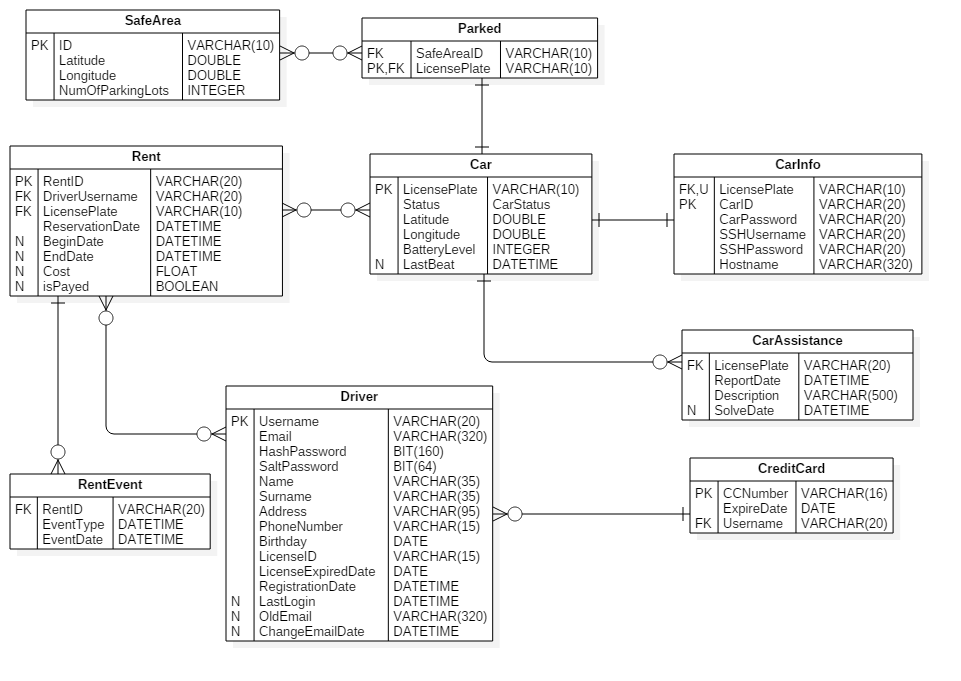
\includegraphics[width=\textwidth, keepaspectratio]{diagrams/Relational.png}
	\caption{Relational model of the database schema.}
	\label {fig:relational}
\end{figure}

Several triggers are implemented to manage some exceptions. For instance:
\begin{itemize}
	\item the registration is cancelled if a driver has never logged into the system in 10 days since his/her registration.
	\item the rent is aborted if a driver doesn't unlock the reserved car within 1 hour. Rental cost is setted to 1 euro.
	\item a report of assistance to a car is generated if more than 10 minutes have passed from the last car heartbeat.
\end{itemize}

\subsubsection{Application server}

The application server runs on a GlassFish server and it's implemented using Servlets. 

The business logic is implemented by custom-built EJB. Given that the state of users, cars and rents is stored in the database, all the EJB are stateless.

Session Beans used for the application server are shown in~\autoref{fig:session-beans}.

\begin{description}
	\item[DriverManager:] manages all the user management features: user registration, user deletion, user profile editing and user salt bytes retrieving.
User registration provides a function that sends an email, with a password and some guidelines, after the registration.
	\item[LogbookManager:] allows users to fetch the history of their past rents.
	\item[SearchCarManager:] allows users to get information about the nearby available cars.
	\item[DriverRentalManager:] allows users to reserve cars, to unlock reserved cars and fetch information about the current rents.
	\item[CarHeartbeat:] manages information coming from cars. It also provides a function responsible for locking cars.
	\item[CarRentalManager:] manages rental information.
\end{description}

\begin{figure}[H]
	\centering
	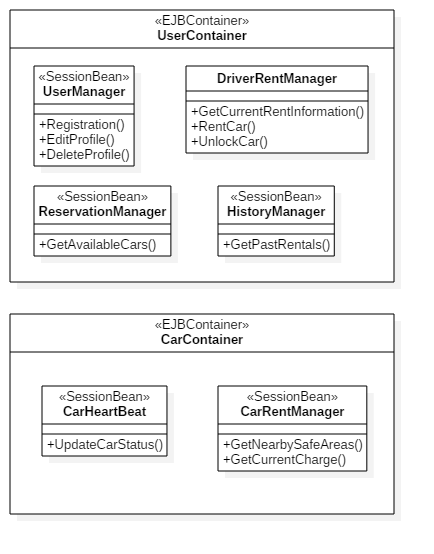
\includegraphics[width=\textwidth, keepaspectratio]{diagrams/SEJBs.png}
	\caption{Session EJBs implemented server side.}
	\label {fig:session-beans}
\end{figure}

The access to the DBMS is not implemented with direct SQL queries: instead, it is completely wrapped by the JPA. The object-relation mapping is done by entity beans. They are simple java classes without a constructor and fulfilled by getter and setter methods for each attributes, that correspond to fields of a database table.

FARE CLASSI UML

\subsubsection{Web server}

The web server runs on GlassFish server. It's implemented using JSP; java EE web components useful when the goal of the web server is to translate RESTful API requests/responses into  HTTP/HTTPS requests/responses. Thanks to JSPs, developers can focusing better on the GUI.

The API requests are managed by a translator, a stateless EJB that simplify the JSP job translating methods calls into API calls.


\begin{figure}[H]
	\centering
	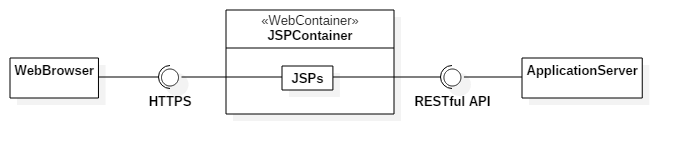
\includegraphics[width=\textwidth, keepaspectratio]{diagrams/WebComponents.png}
	\caption{The components and the interfaces of the web tier.}
	\label {fig:web-components}
\end{figure}

Even if REST is a stateless architectural style, JSPs lead users to a stateful communication saving the session in order to avoid further insertion of user's credentials.

\subsubsection{Car computer}

Every car hosts a computer with a linux distribution of Ubuntu 16.10 as operating system. In any OS is installed openssh-server, in order to access to the car remotly, and two applications:
\begin{description}
	\item[Heartbeat:] this application is always running and sends, every 10 seconds, information about the current status, of both car and rent, to the application server through a single API call. The application server will ignore the rental information if the car is not rented.
	\item[CarGUI:] this application is started everytime the car gets unlocked, and closed everytime the car gets locked. It asks, through API calls, for user information, user's current charges and nearby availabe safe areas, in order to display those information on the GUI.
\end{description}

\begin{figure}[H]
	\centering
	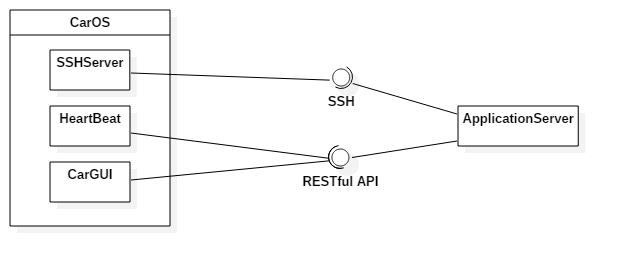
\includegraphics[width=\textwidth, keepaspectratio]{diagrams/CarClientComponents.png}
	\caption{The components and the interfaces of the car client tier.}
	\label {fig:car-client-components}
\end{figure}

\subsubsection{Mobile application}

The mobile client implementation depends on the specific platform. 
The iOS application is implemented in Swift and mainly uses UIKit framework to manage the UI interface.
Instead, the Android application is implemented in Java and mainly uses android.view package for graphical management.

The application core is composed by a controller which translates the inputs from the UI into remote functions calls via  RESTful APIs. The controller also manages the interaction with the GPS component using  CoreLocation framework in iOS app and LocationListener interface in the Android one.

\begin{figure}[H]
    \centering
    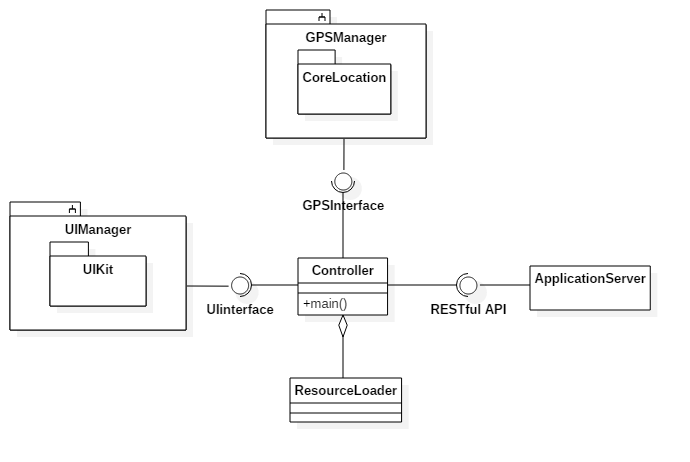
\includegraphics[width=\textwidth, keepaspectratio]{diagrams/iOS.png}
    \caption{The components of the iOS application.}
    \label{fig:ios-app}
\end{figure}

\begin{figure}[H]
    \centering
    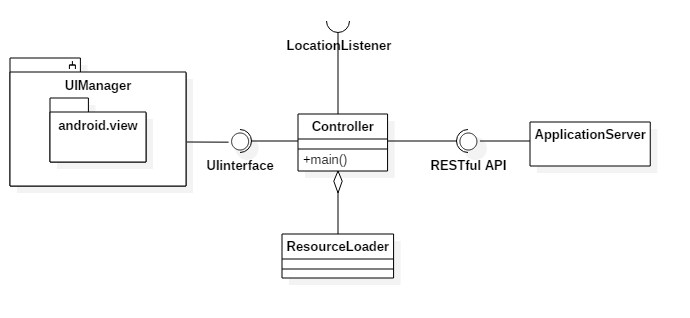
\includegraphics[width=\textwidth, keepaspectratio]{diagrams/Android.png}
    \caption{The components of the Android application.}
    \label{fig:android-app}
\end{figure}

\subsection{Deployment view}

The deployment diagram for the system is shown in~\autoref{fig:deployment}.

\begin{figure}[H]
	\centering
	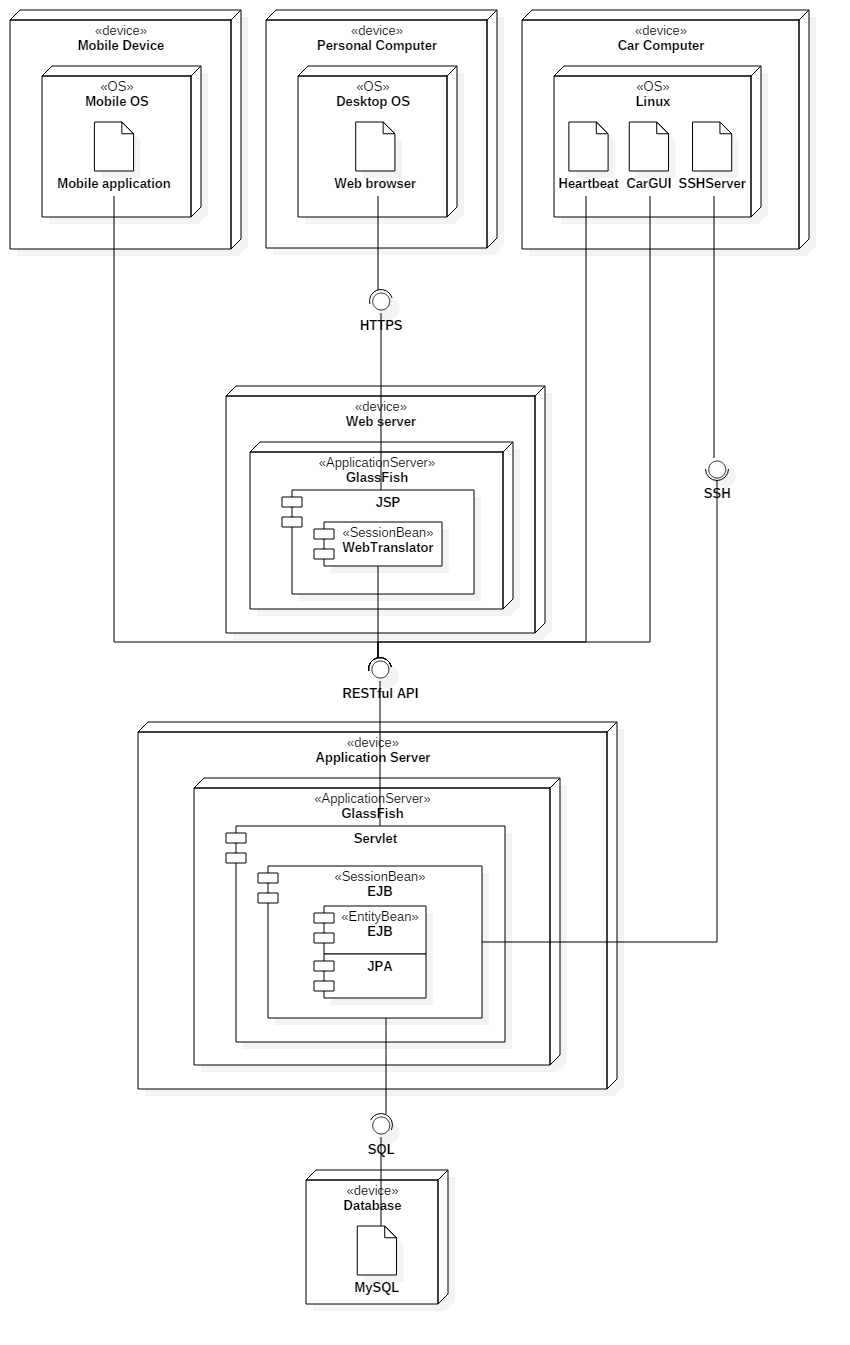
\includegraphics[height=500px, keepaspectratio]{diagrams/Deployment.png}
	\caption{The deployment diagram of the PowerEnJoy system.}
	\label {fig:deployment}
\end{figure}

\subsection{Component interfaces}

\subsubsection{Application server to database}

The application server communicates with the DBMS via the Java Persistence API over standard network protocols.

The low-level technicalities about the specific dialect of SQL for the selected DBMS are abstracted by the Java Persistence API, which also deals with the O/R mapping.

\subsubsection{Application server to cars}

The application server communicates with the cars through the SSHv2 protocol. It provides an encrypted and remote communication over the standard network.

The credentials used for the remote access are stored in the database as plaintext and different for each car. There is no reason to protect the credentials hashing and/or salting them, because it won't add any security measure.

\subsubsection{Front-ends to application server (API)}

As already said, the front-ends applications communicate with the application server through RESTful API over the HTTPS protocol. They are provided by the application server and use JSON as data representation language.

The detailed RESTful API is described in the following pages. 

\bigskip

\noindent Common to all the requests:
\begin{itemize}
	\item the paths must be applied to the application server domain.
	\item a 422 error means that the JSON object has been not created correctly or the values of the objects' fields cannot be processed by the application server. For instance, the username choosen could be already taken or could not match to the regular expression choosen by the system.
	\item requests over HTTP protocol are denied.
\end{itemize}
Requests processed by cars also require an authentication process in order to avoid fake requests from unknown entities. As already said for the SSH credentials, they are stored in the database as plaintext, diffent for each car and from the SSH credentials.




\subsubsubsection{[User] User creation}
\begin{figure}[H]
	\noindent
    	\centering
    	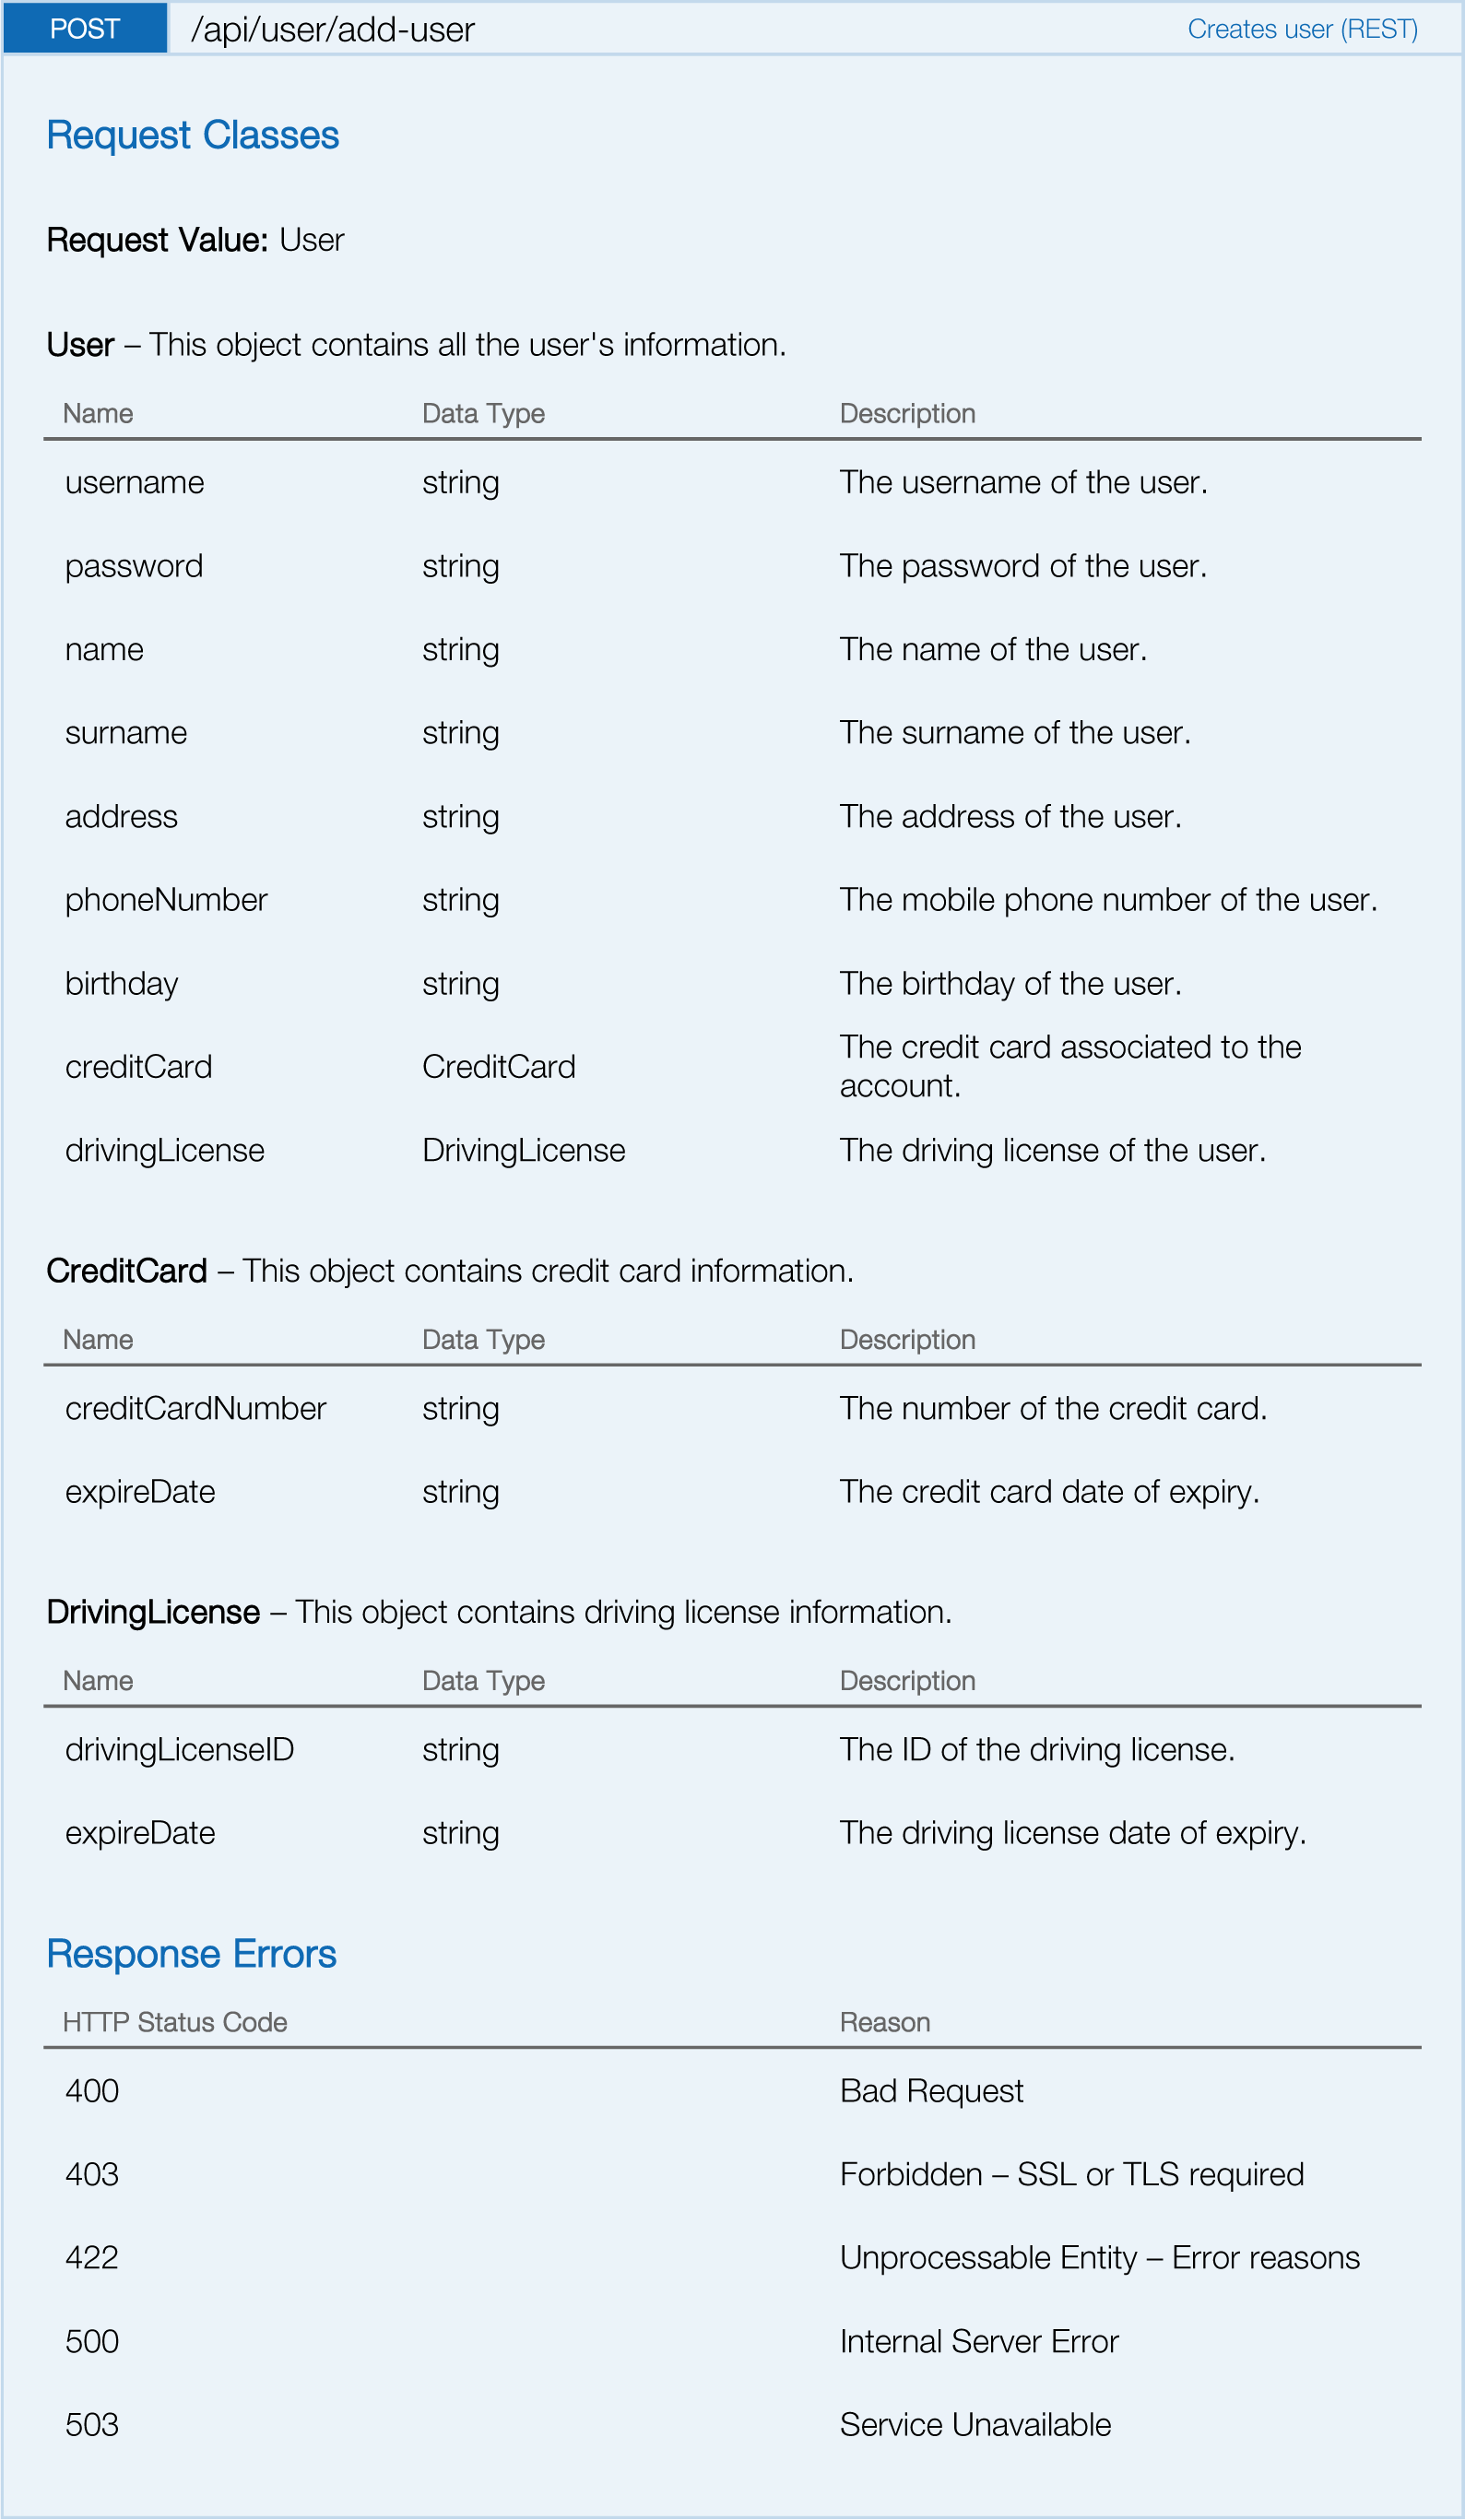
\includegraphics[height=550px, keepaspectratio]{apitables/APIAddUser.png}
    	\label{fig:api-add-user}
\end{figure}

\subsubsubsection{[User] User's salt bytes retrieval}
\begin{figure}[H]
	\noindent
    	\centering
    	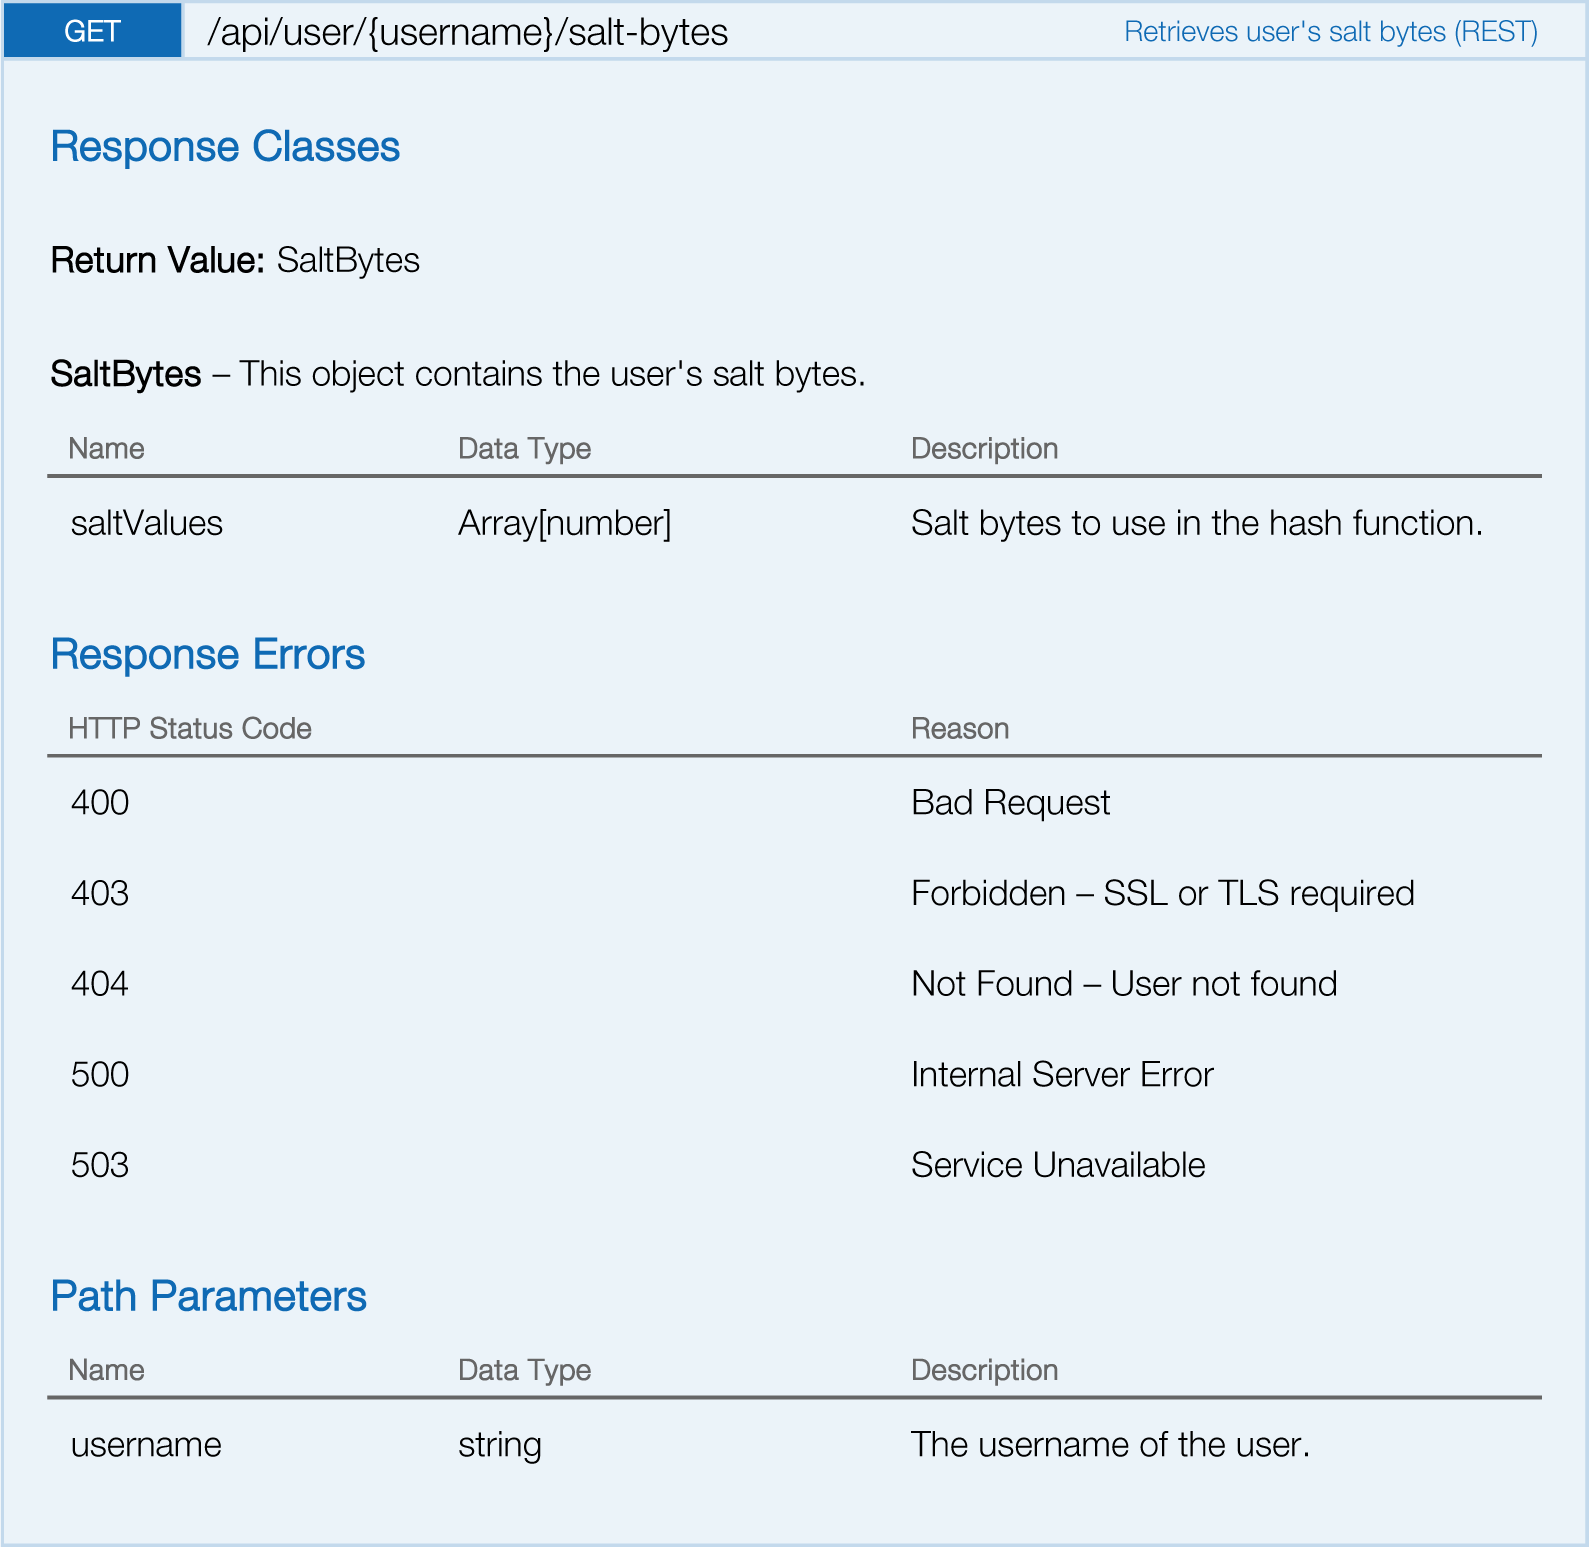
\includegraphics{apitables/APISaltBytes.png}
    	\label{fig:api-salt-bytes}
\end{figure}

\subsubsubsection{[User] User deletion}
\begin{figure}[H]
	\noindent
    	\centering
    	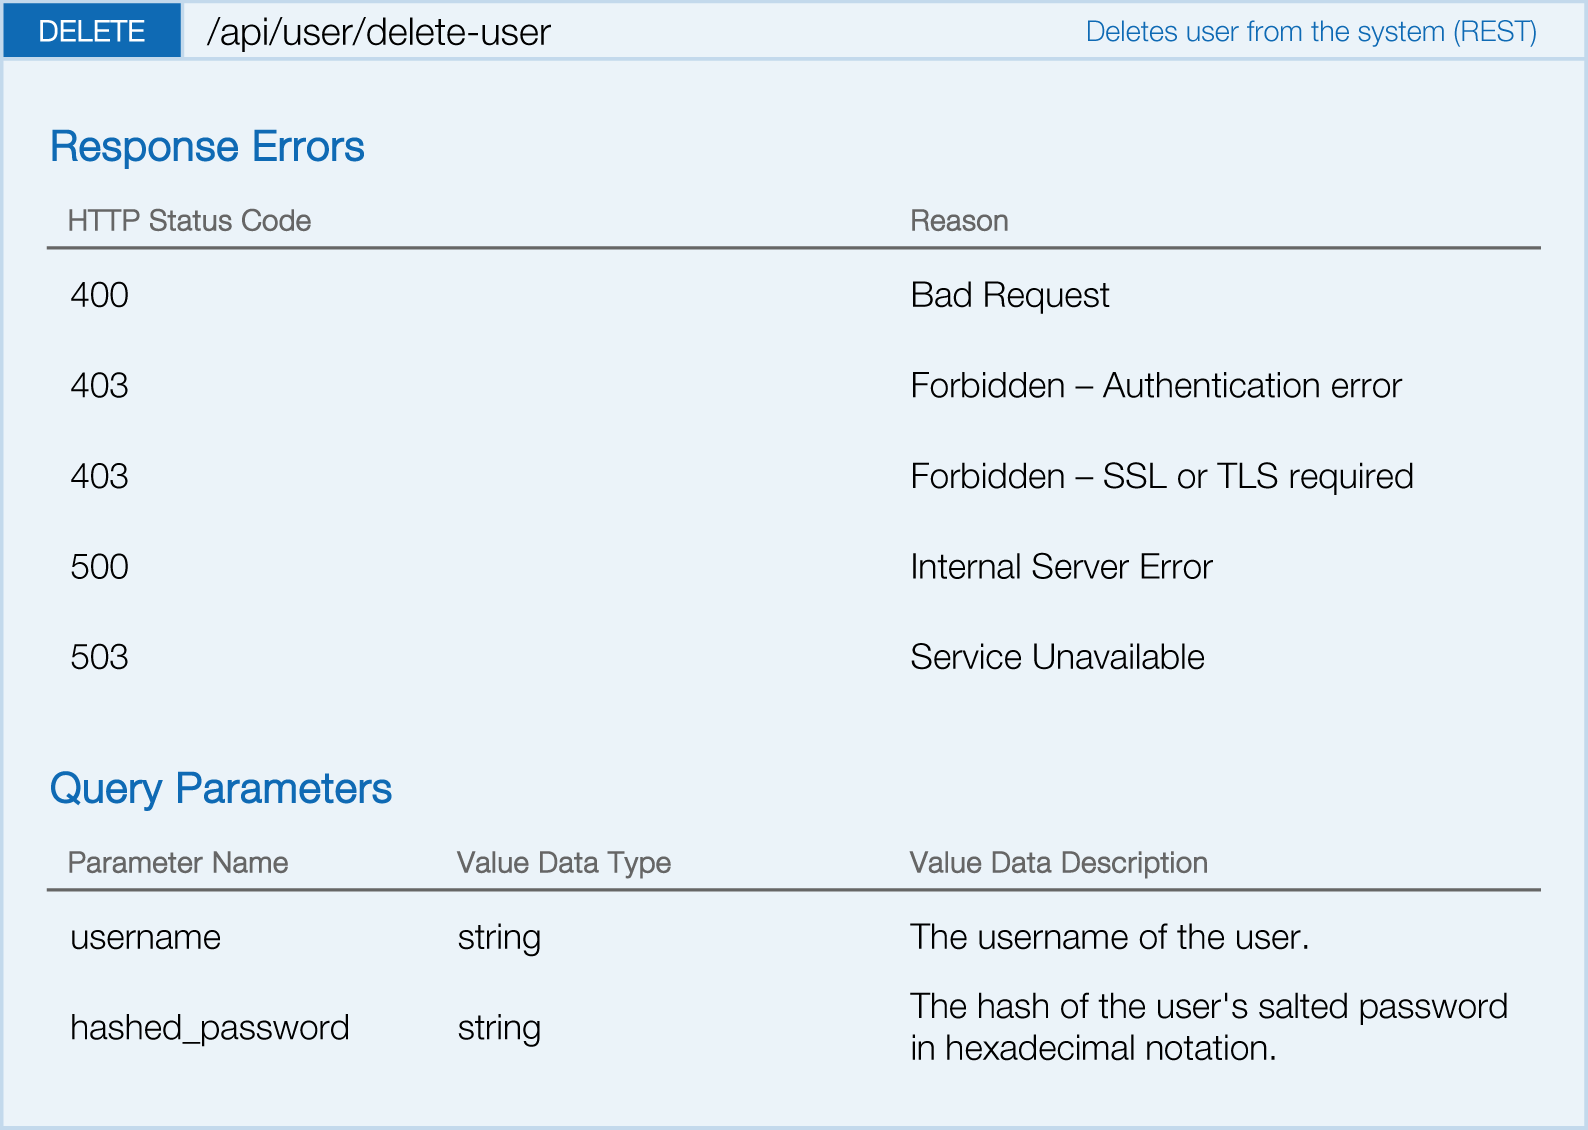
\includegraphics{apitables/APIDeleteUser.png}
    	\label{fig:api-delete-user}
\end{figure}

\subsubsubsection{[User] User's rental logbook retrieval}
\begin{figure}[H]
	\noindent
    	\centering 
    	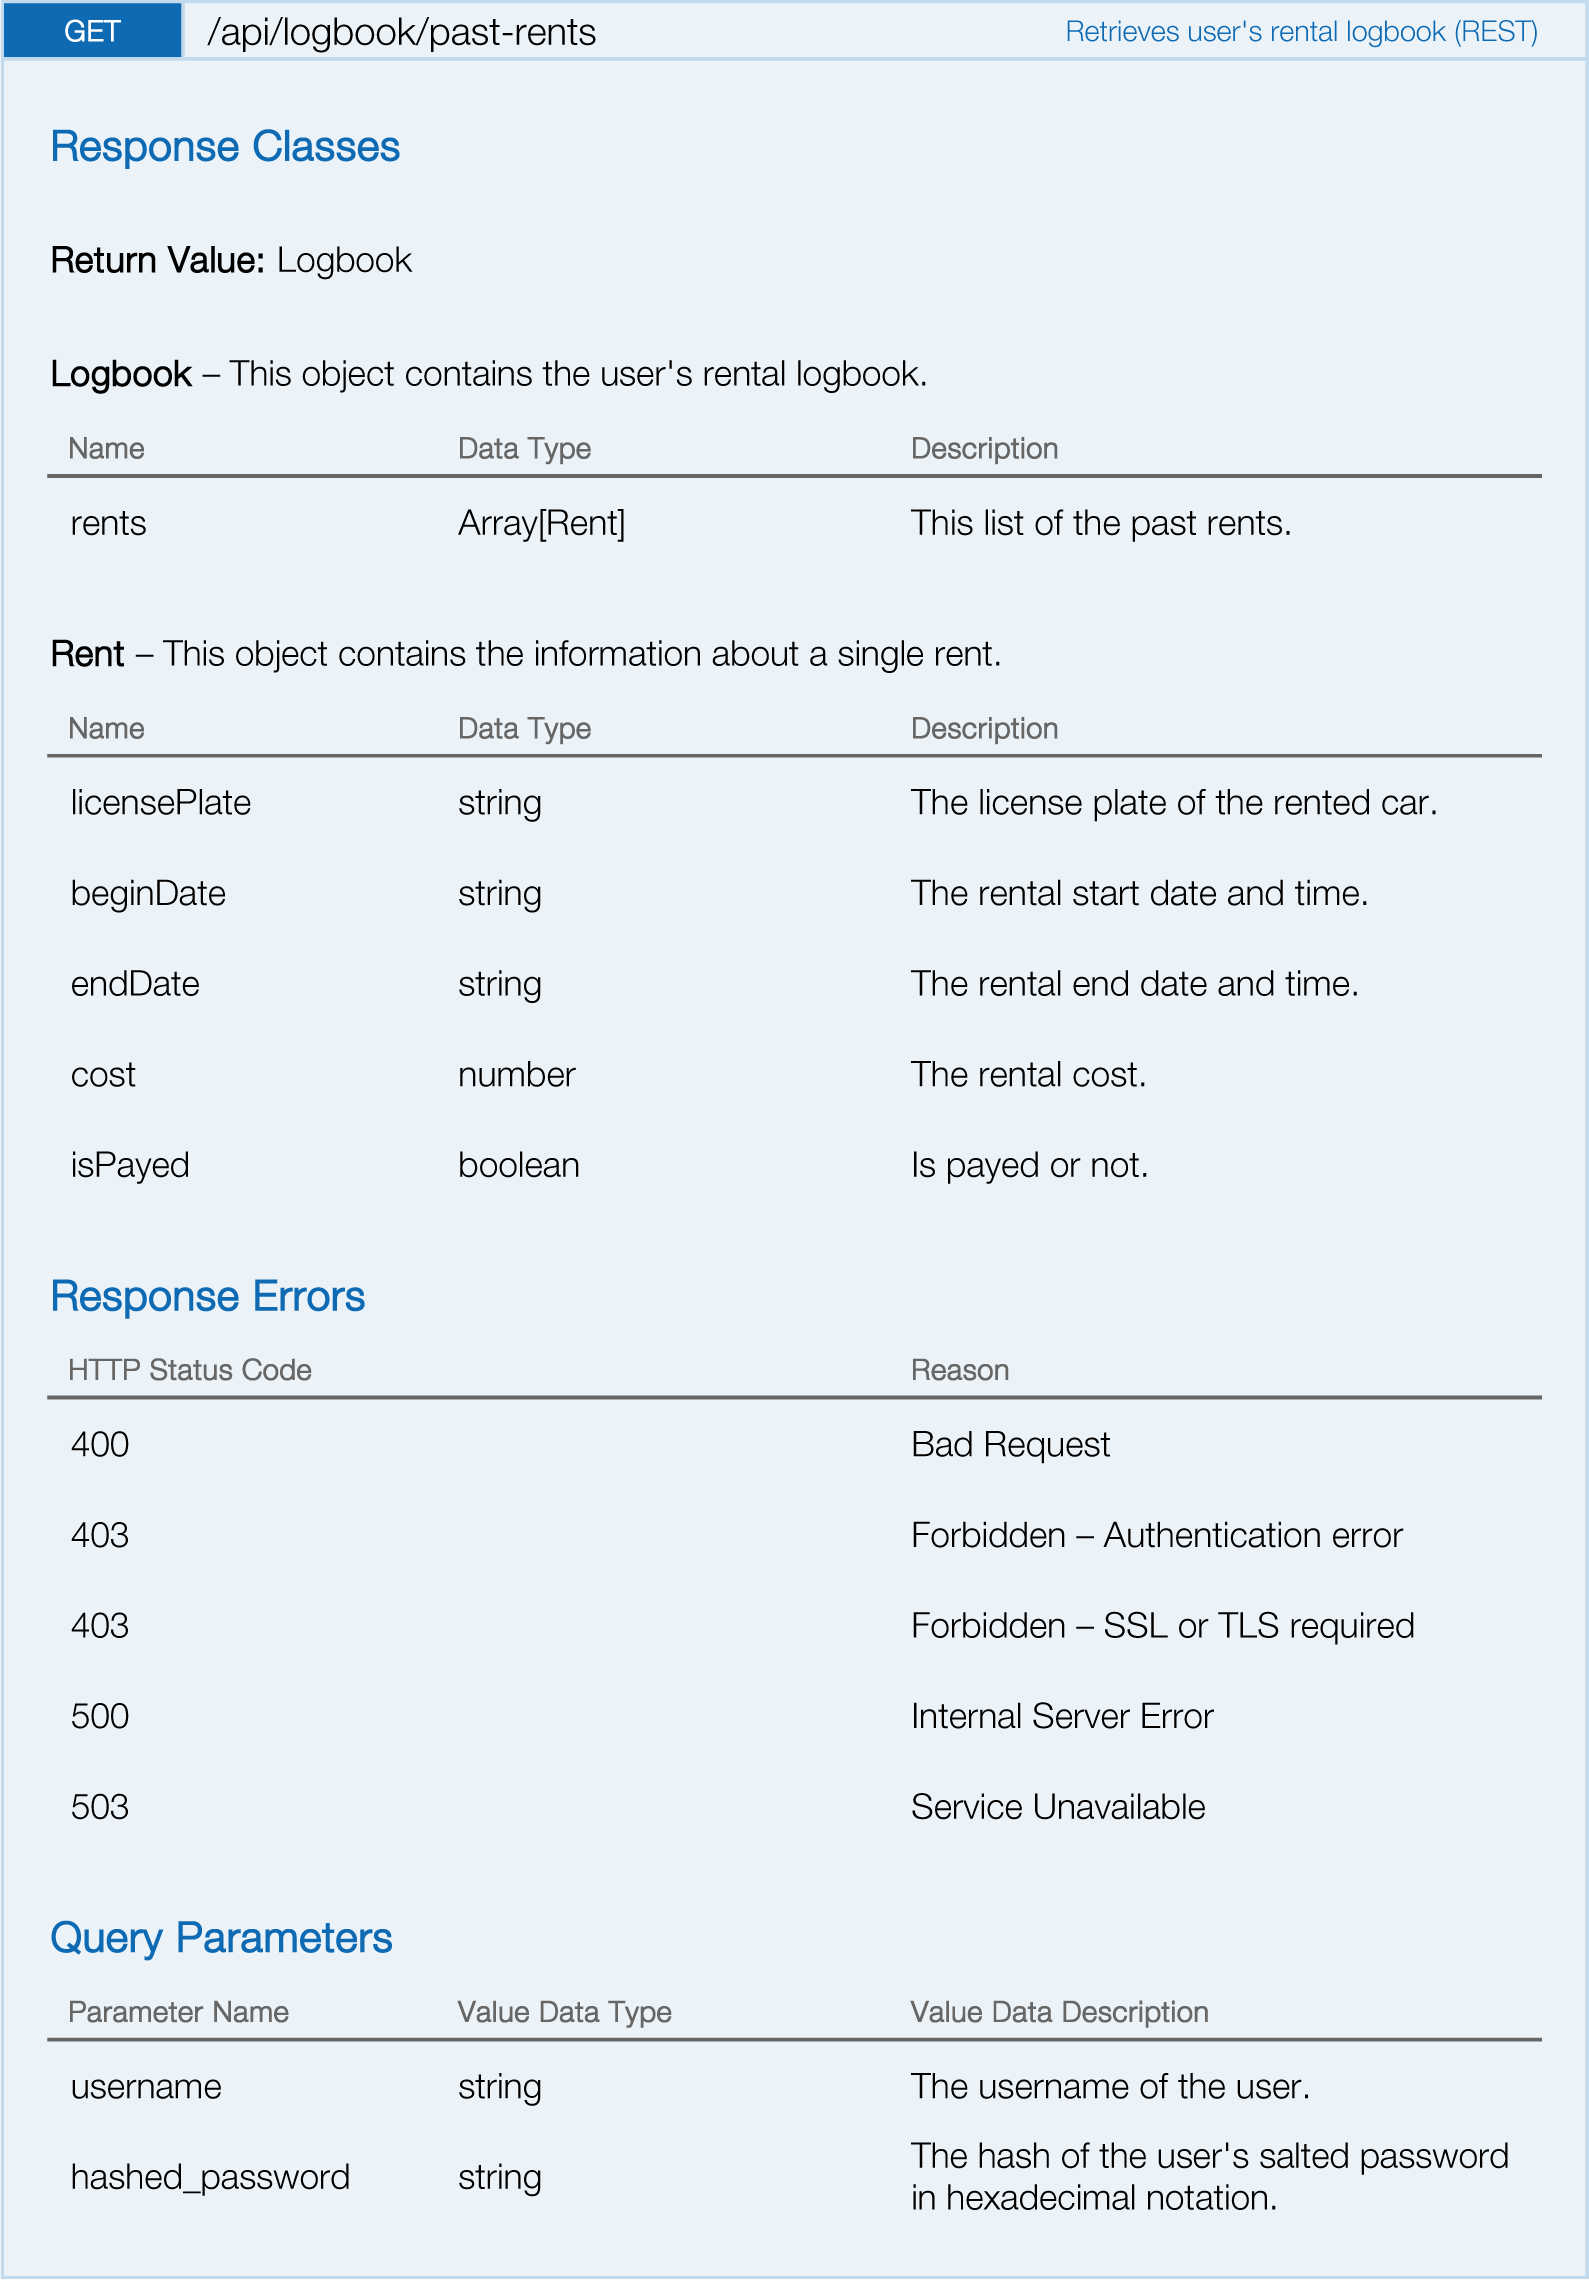
\includegraphics{apitables/APIPastRents.png}
    	\label{fig:api-past-rents}
\end{figure}

\subsubsubsection{[User] Available cars' retrieval}
\begin{figure}[H]
	\noindent
    	\centering
    	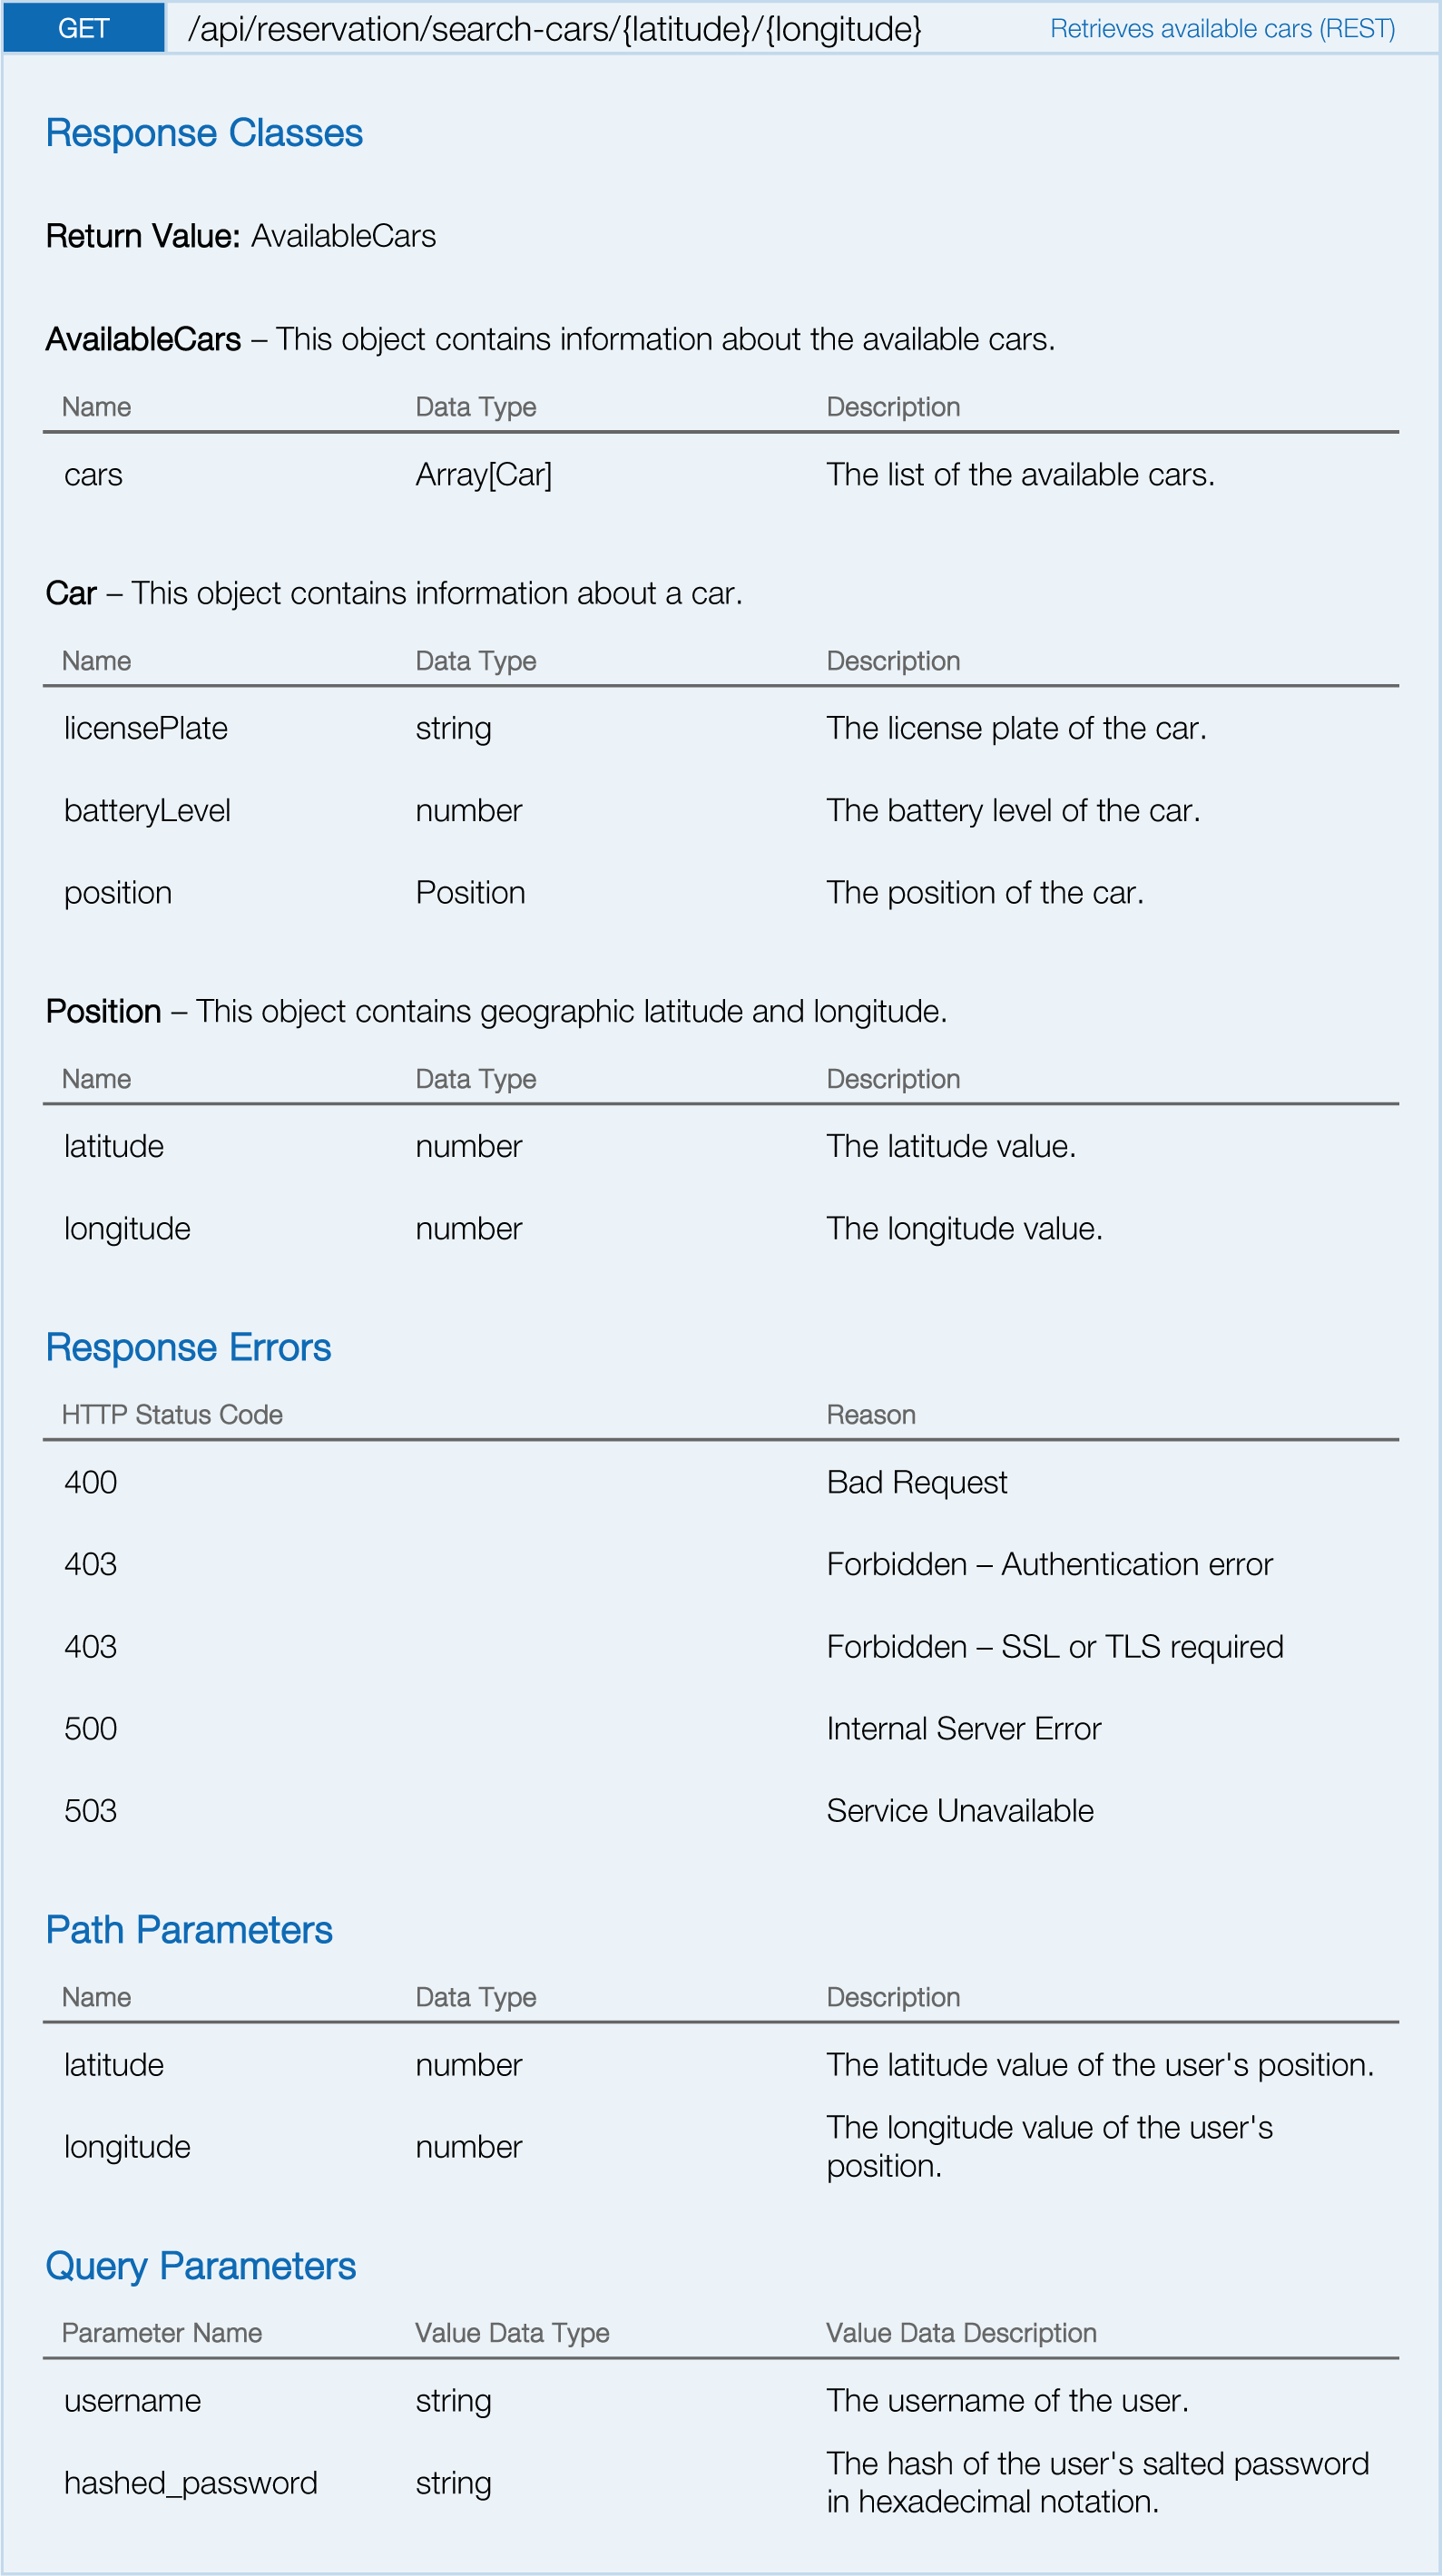
\includegraphics[height=550px, keepaspectratio]{apitables/APISearchCars.png}
    	\label{fig:api-search-cars}
\end{figure}

\subsubsubsection{[User] Car reservation}
\begin{figure}[H]
	\noindent
    	\centering
    	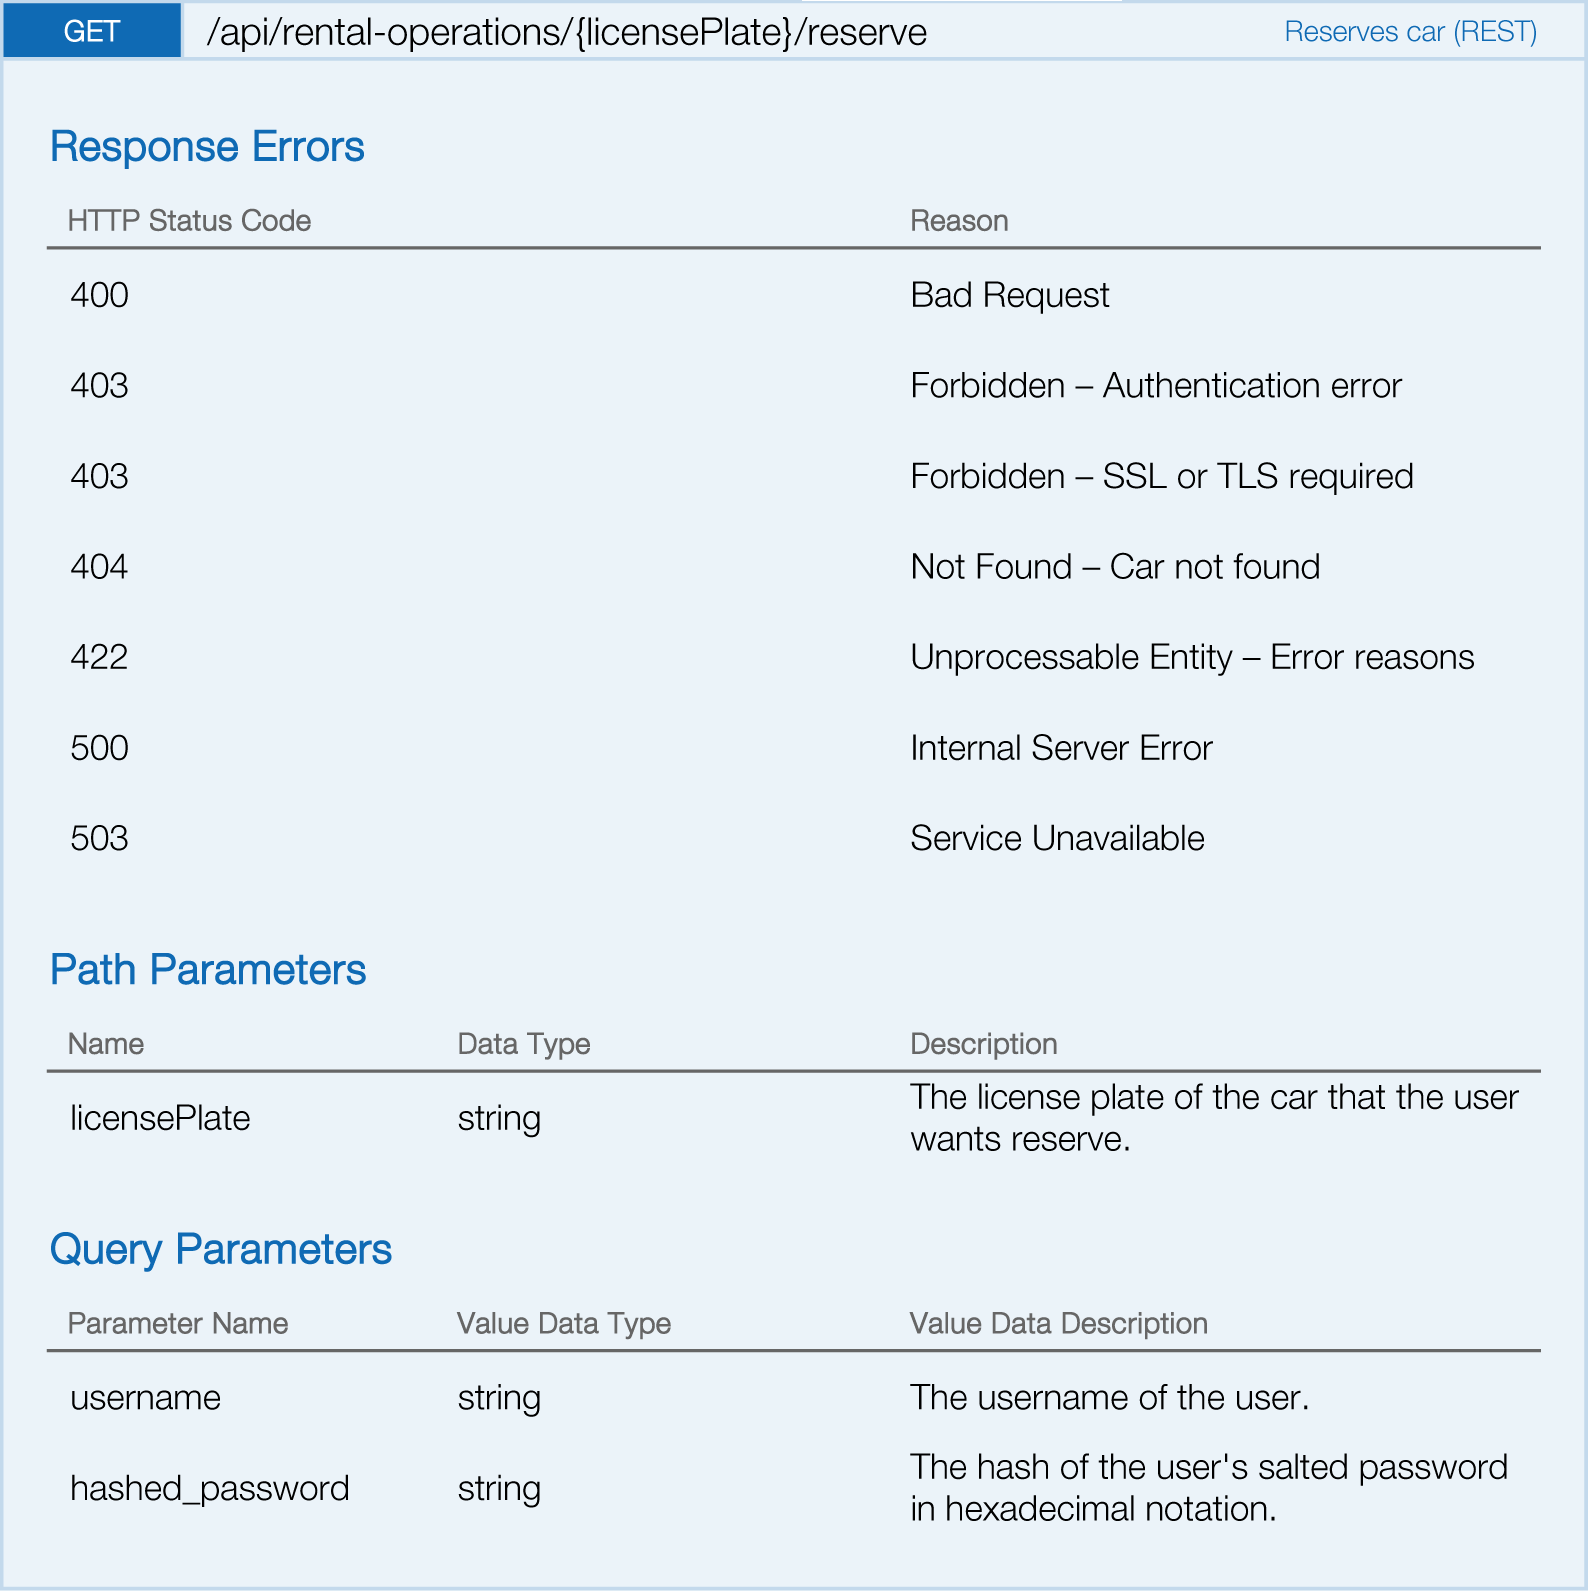
\includegraphics{apitables/APIReservation.png}
    	\label{fig:api-reservation}
\end{figure}

\subsubsubsection{[User] Current reservation retrieval}
\begin{figure}[H]
	\noindent
    	\centering
    	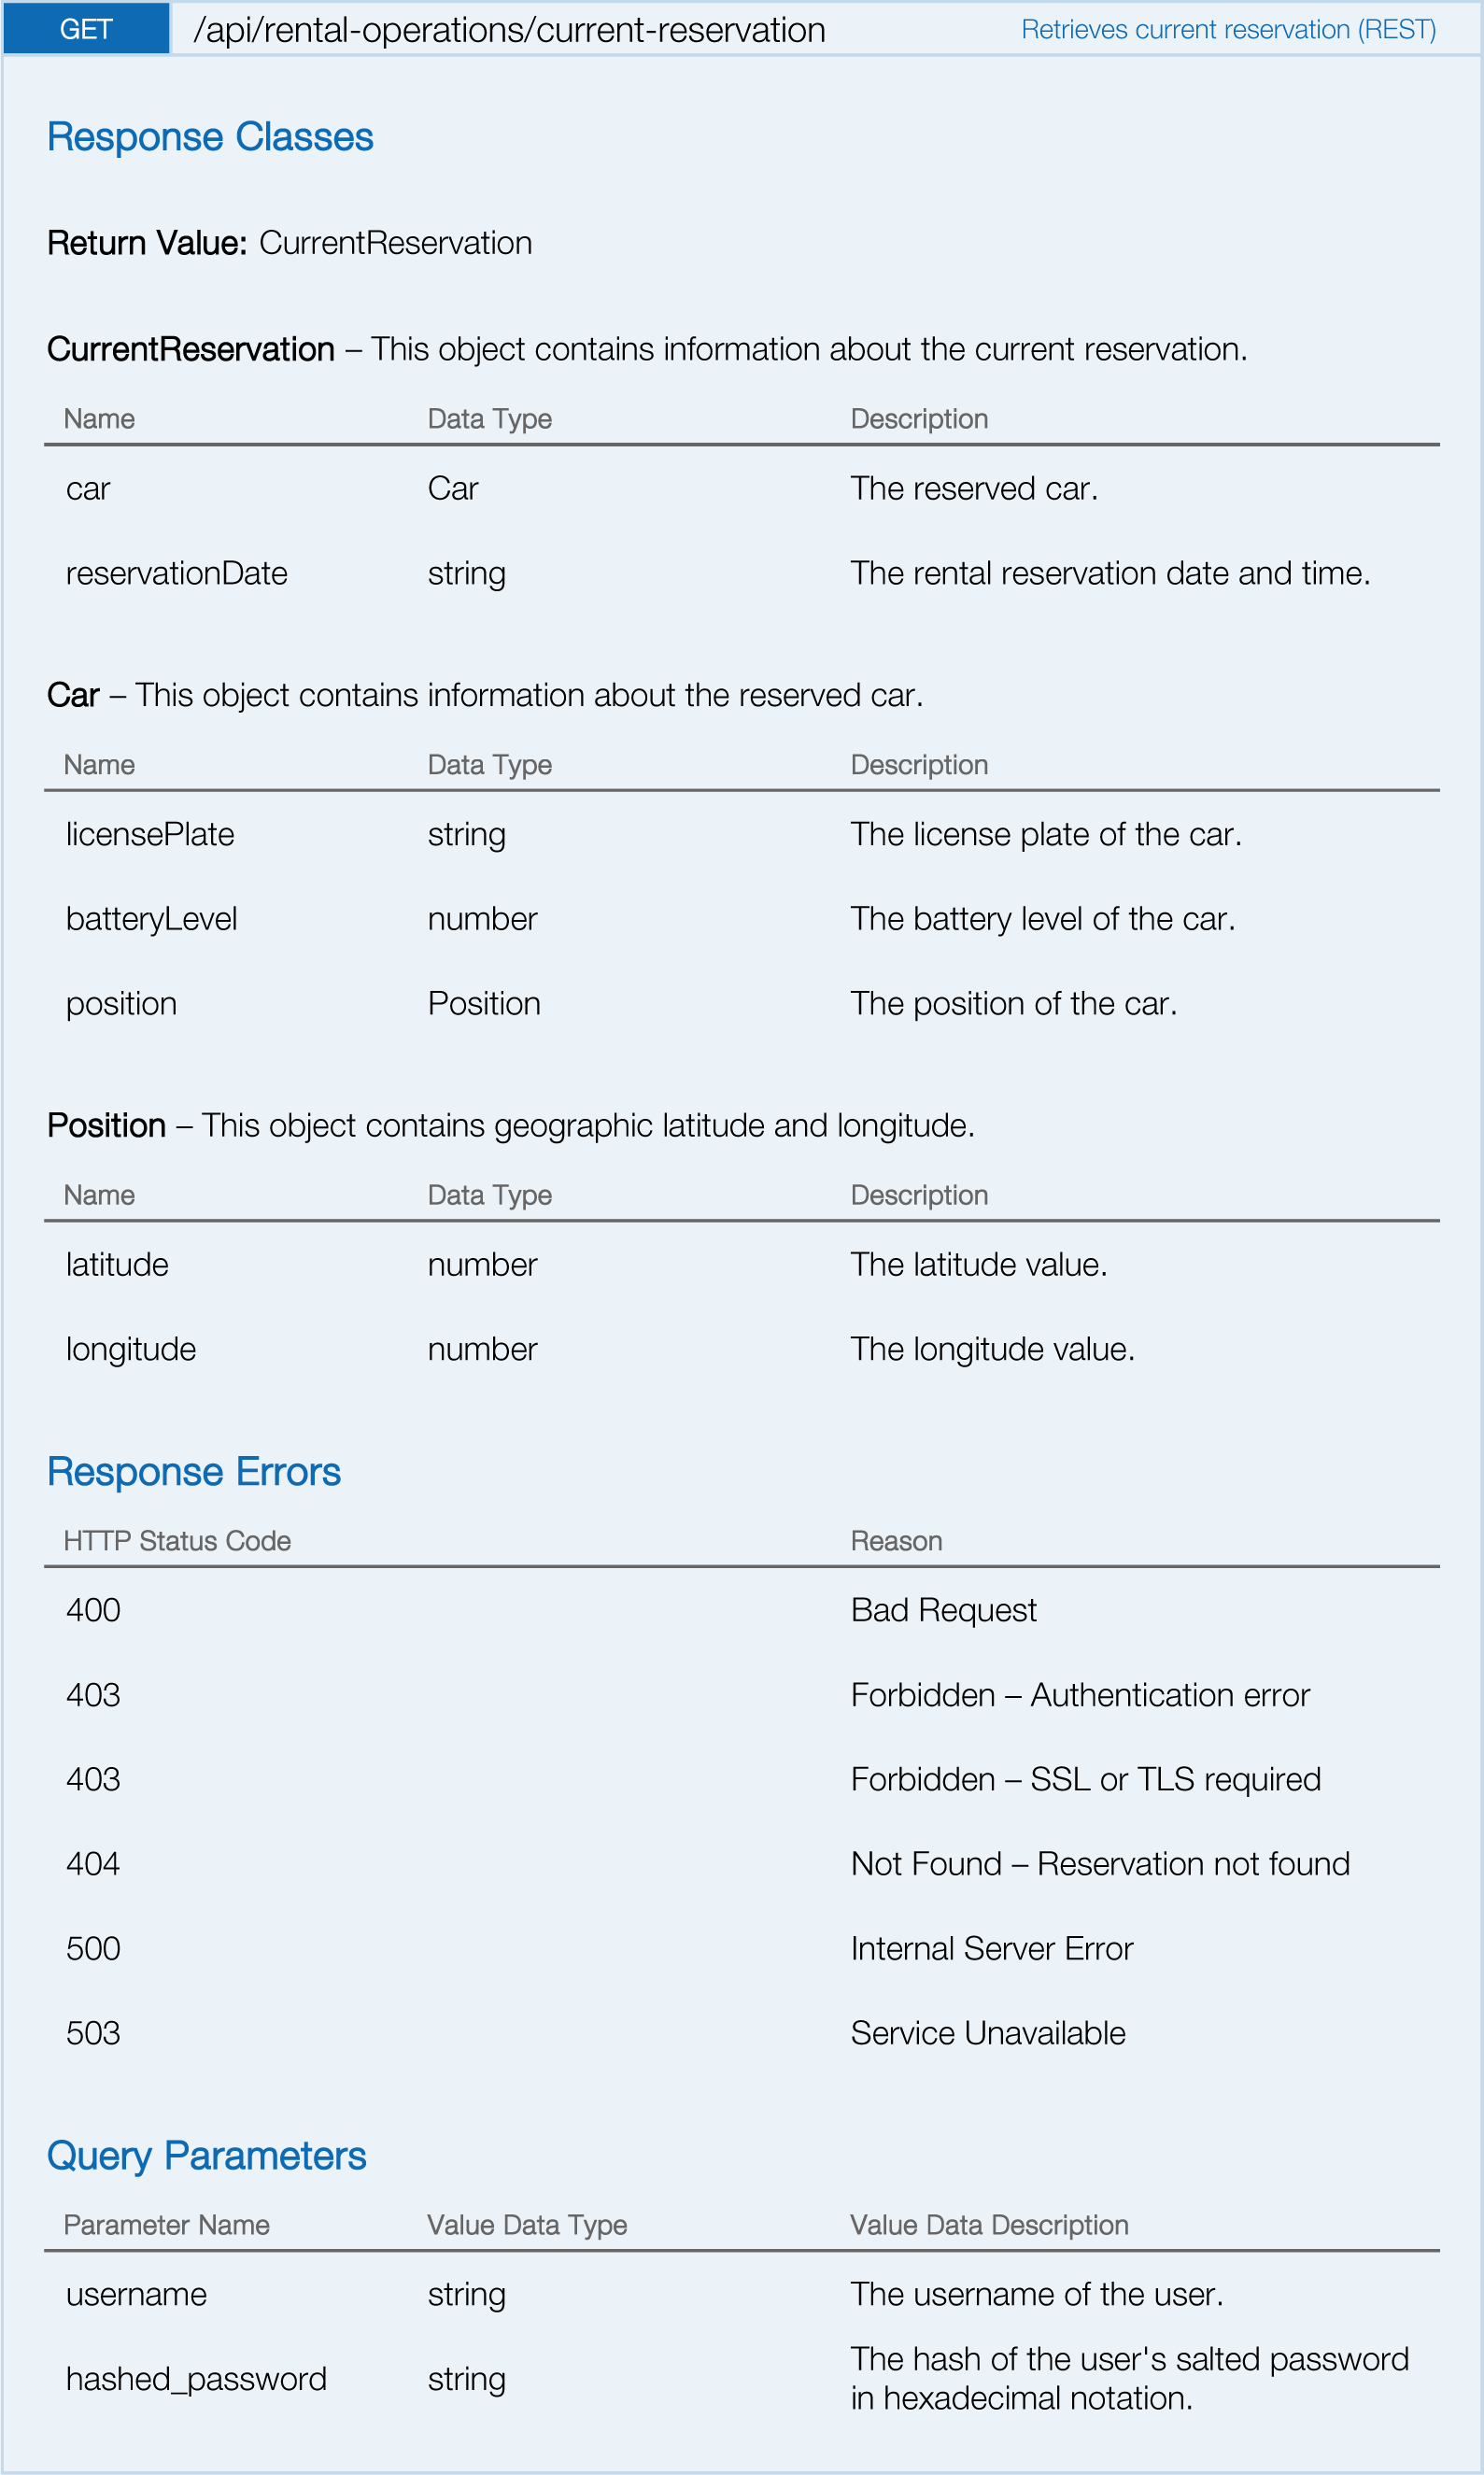
\includegraphics[height=550px, keepaspectratio]{apitables/APICurrentReservation.png}
    	\label{fig:api-current-reservation}
\end{figure}

\subsubsubsection{[User] Unlocks car}
\begin{figure}[H]
	\noindent
    	\centering
    	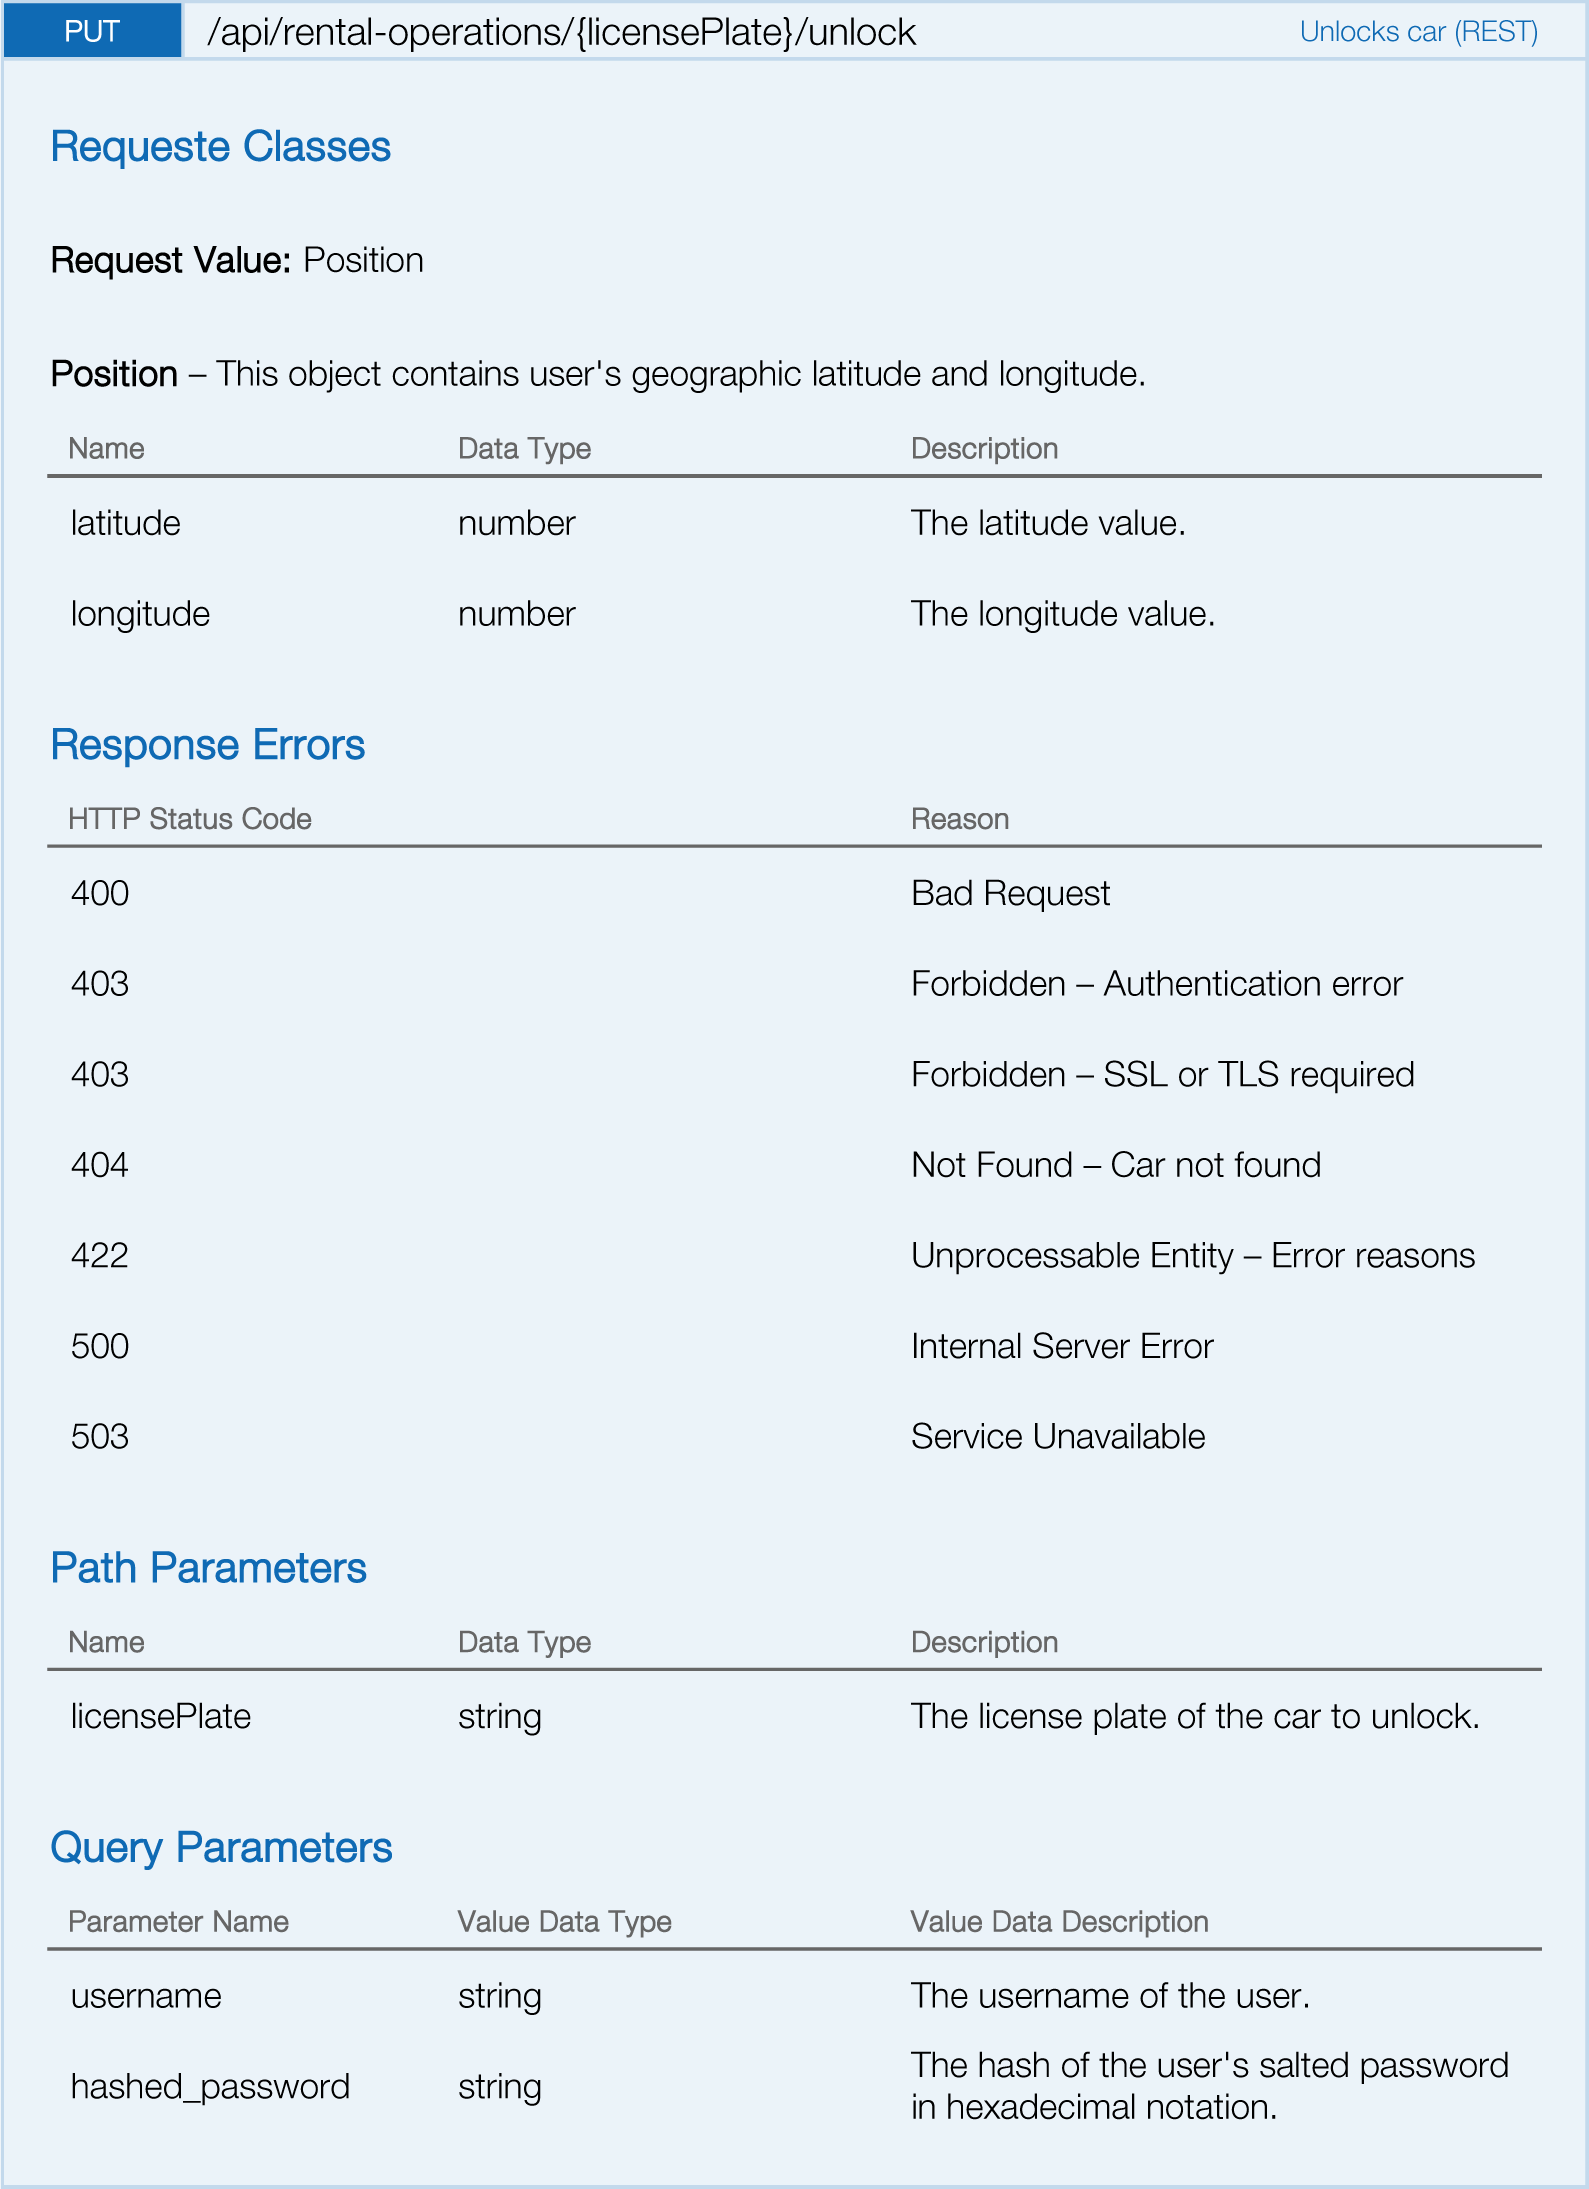
\includegraphics{apitables/APIUnlockCar.png}
    	\label{fig:api-unlock-car}
\end{figure}

\subsubsubsection{[Car] Car Heartbeat}
\begin{figure}[H]
	\noindent
    	\centering
    	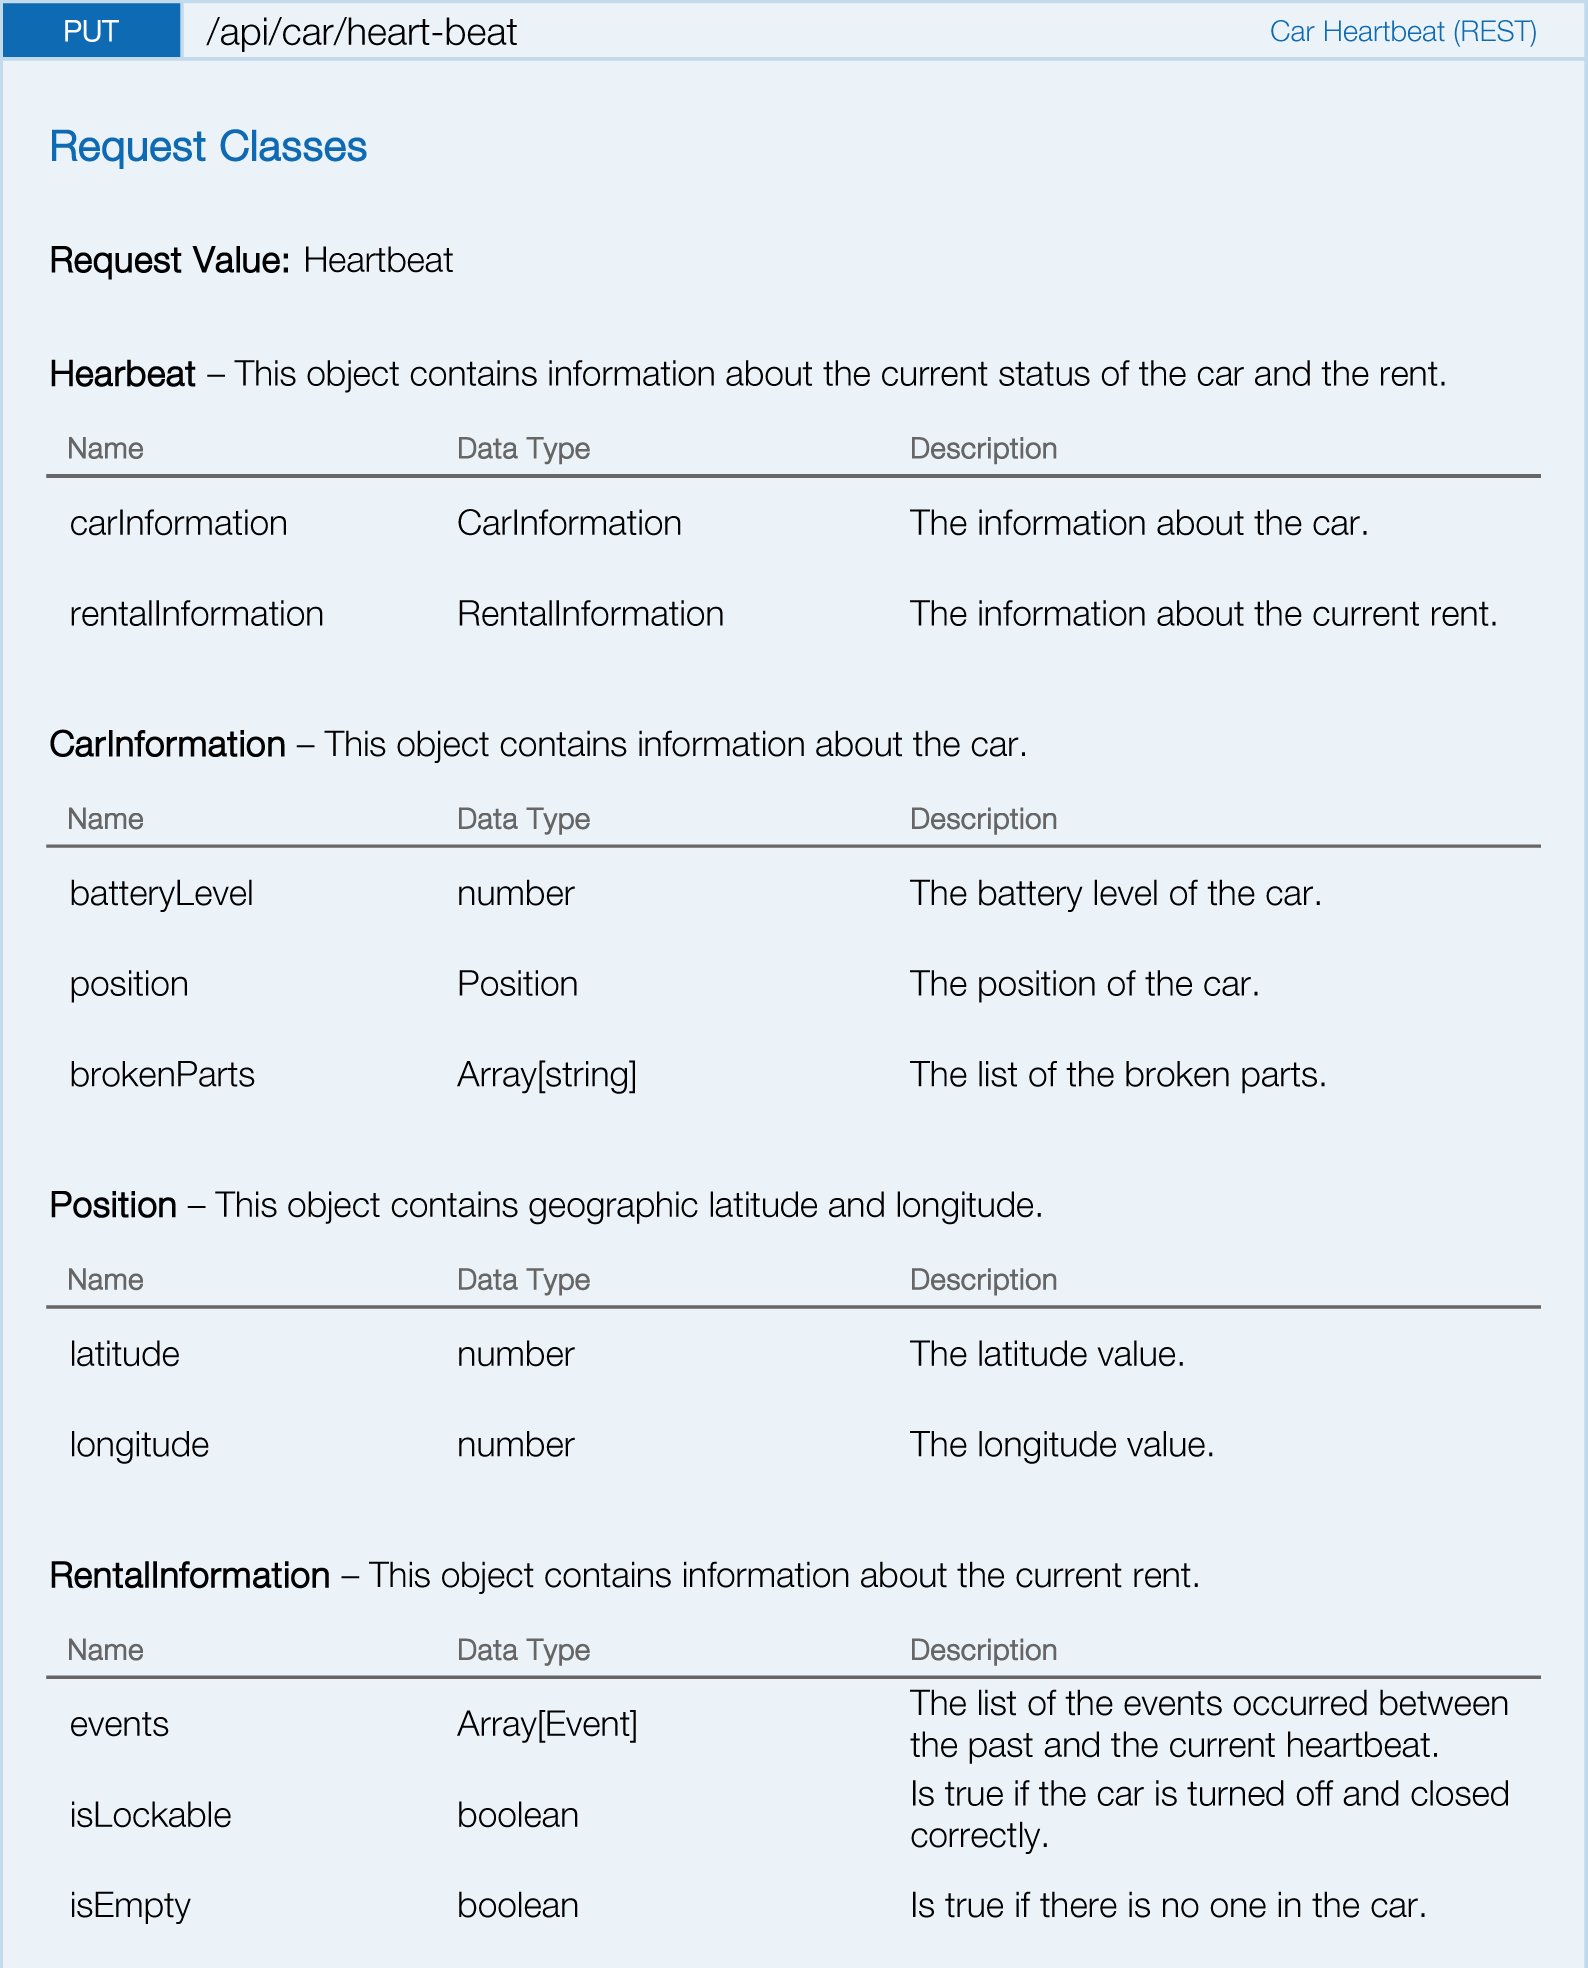
\includegraphics{apitables/APIHeartbeat1.png}
    	\label{fig:api-car-heartbeat1}
\end{figure}

\begin{figure}[H]
	\noindent
    	\centering
    	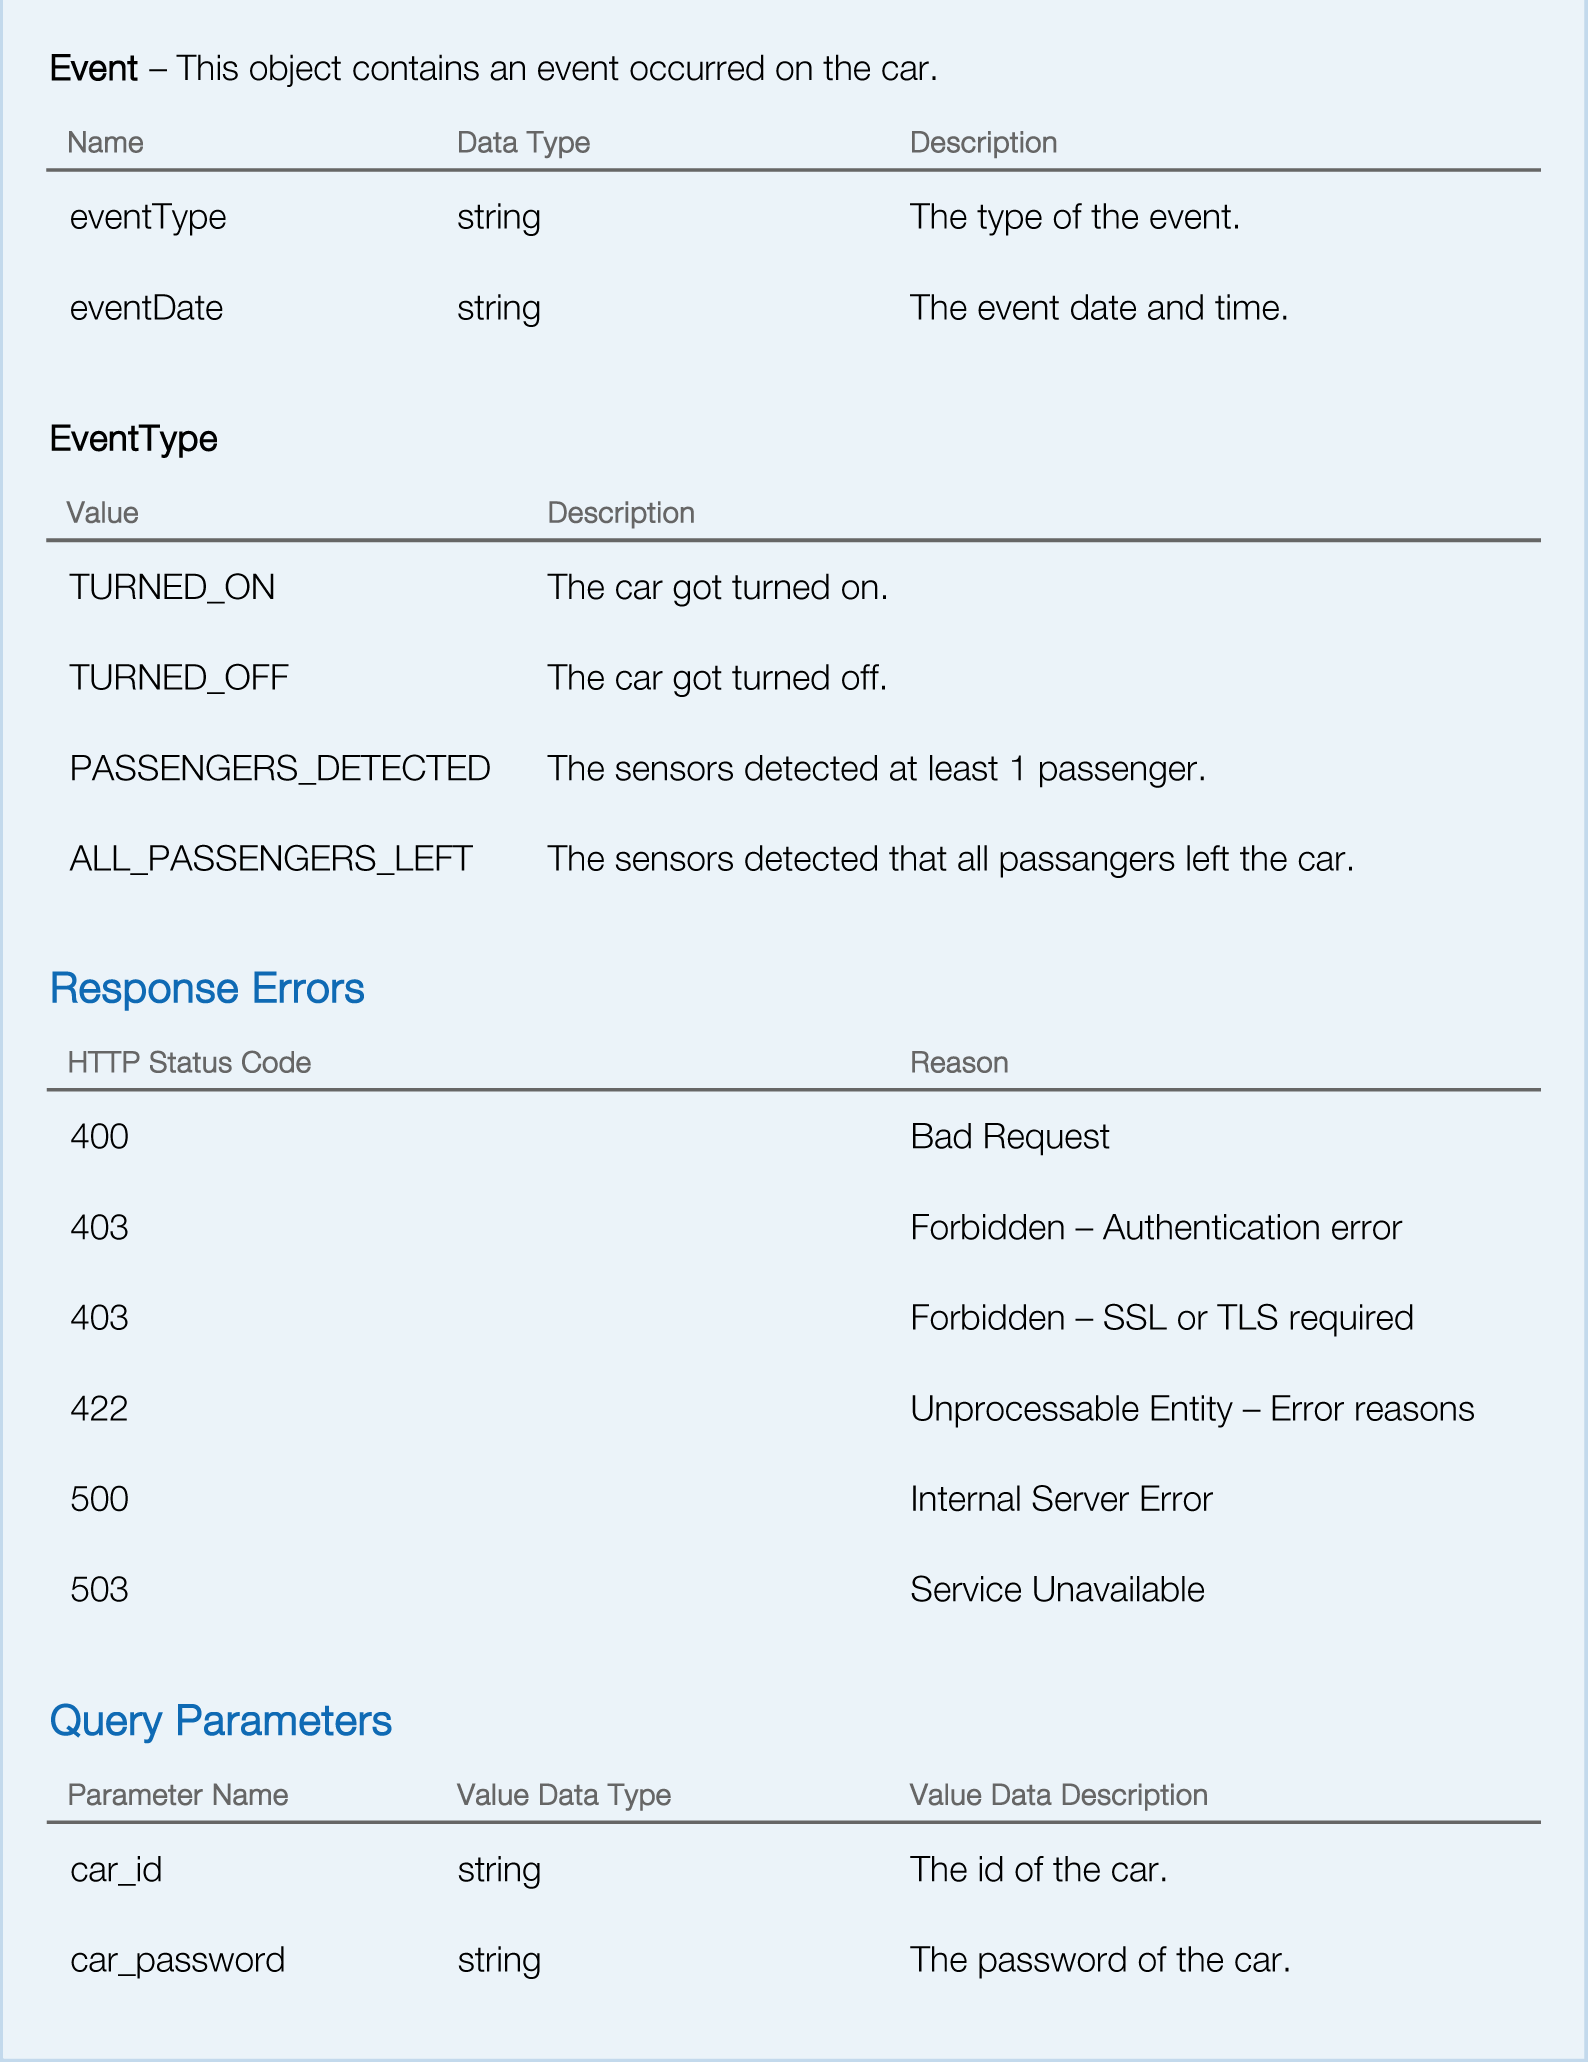
\includegraphics{apitables/APIHeartbeat2.png}
    	\label{fig:api-car-heartbeat2}
\end{figure}

\subsubsubsection{[Car] Available safe areas' retrieval}
\begin{figure}[H]
	\noindent
    	\centering
    	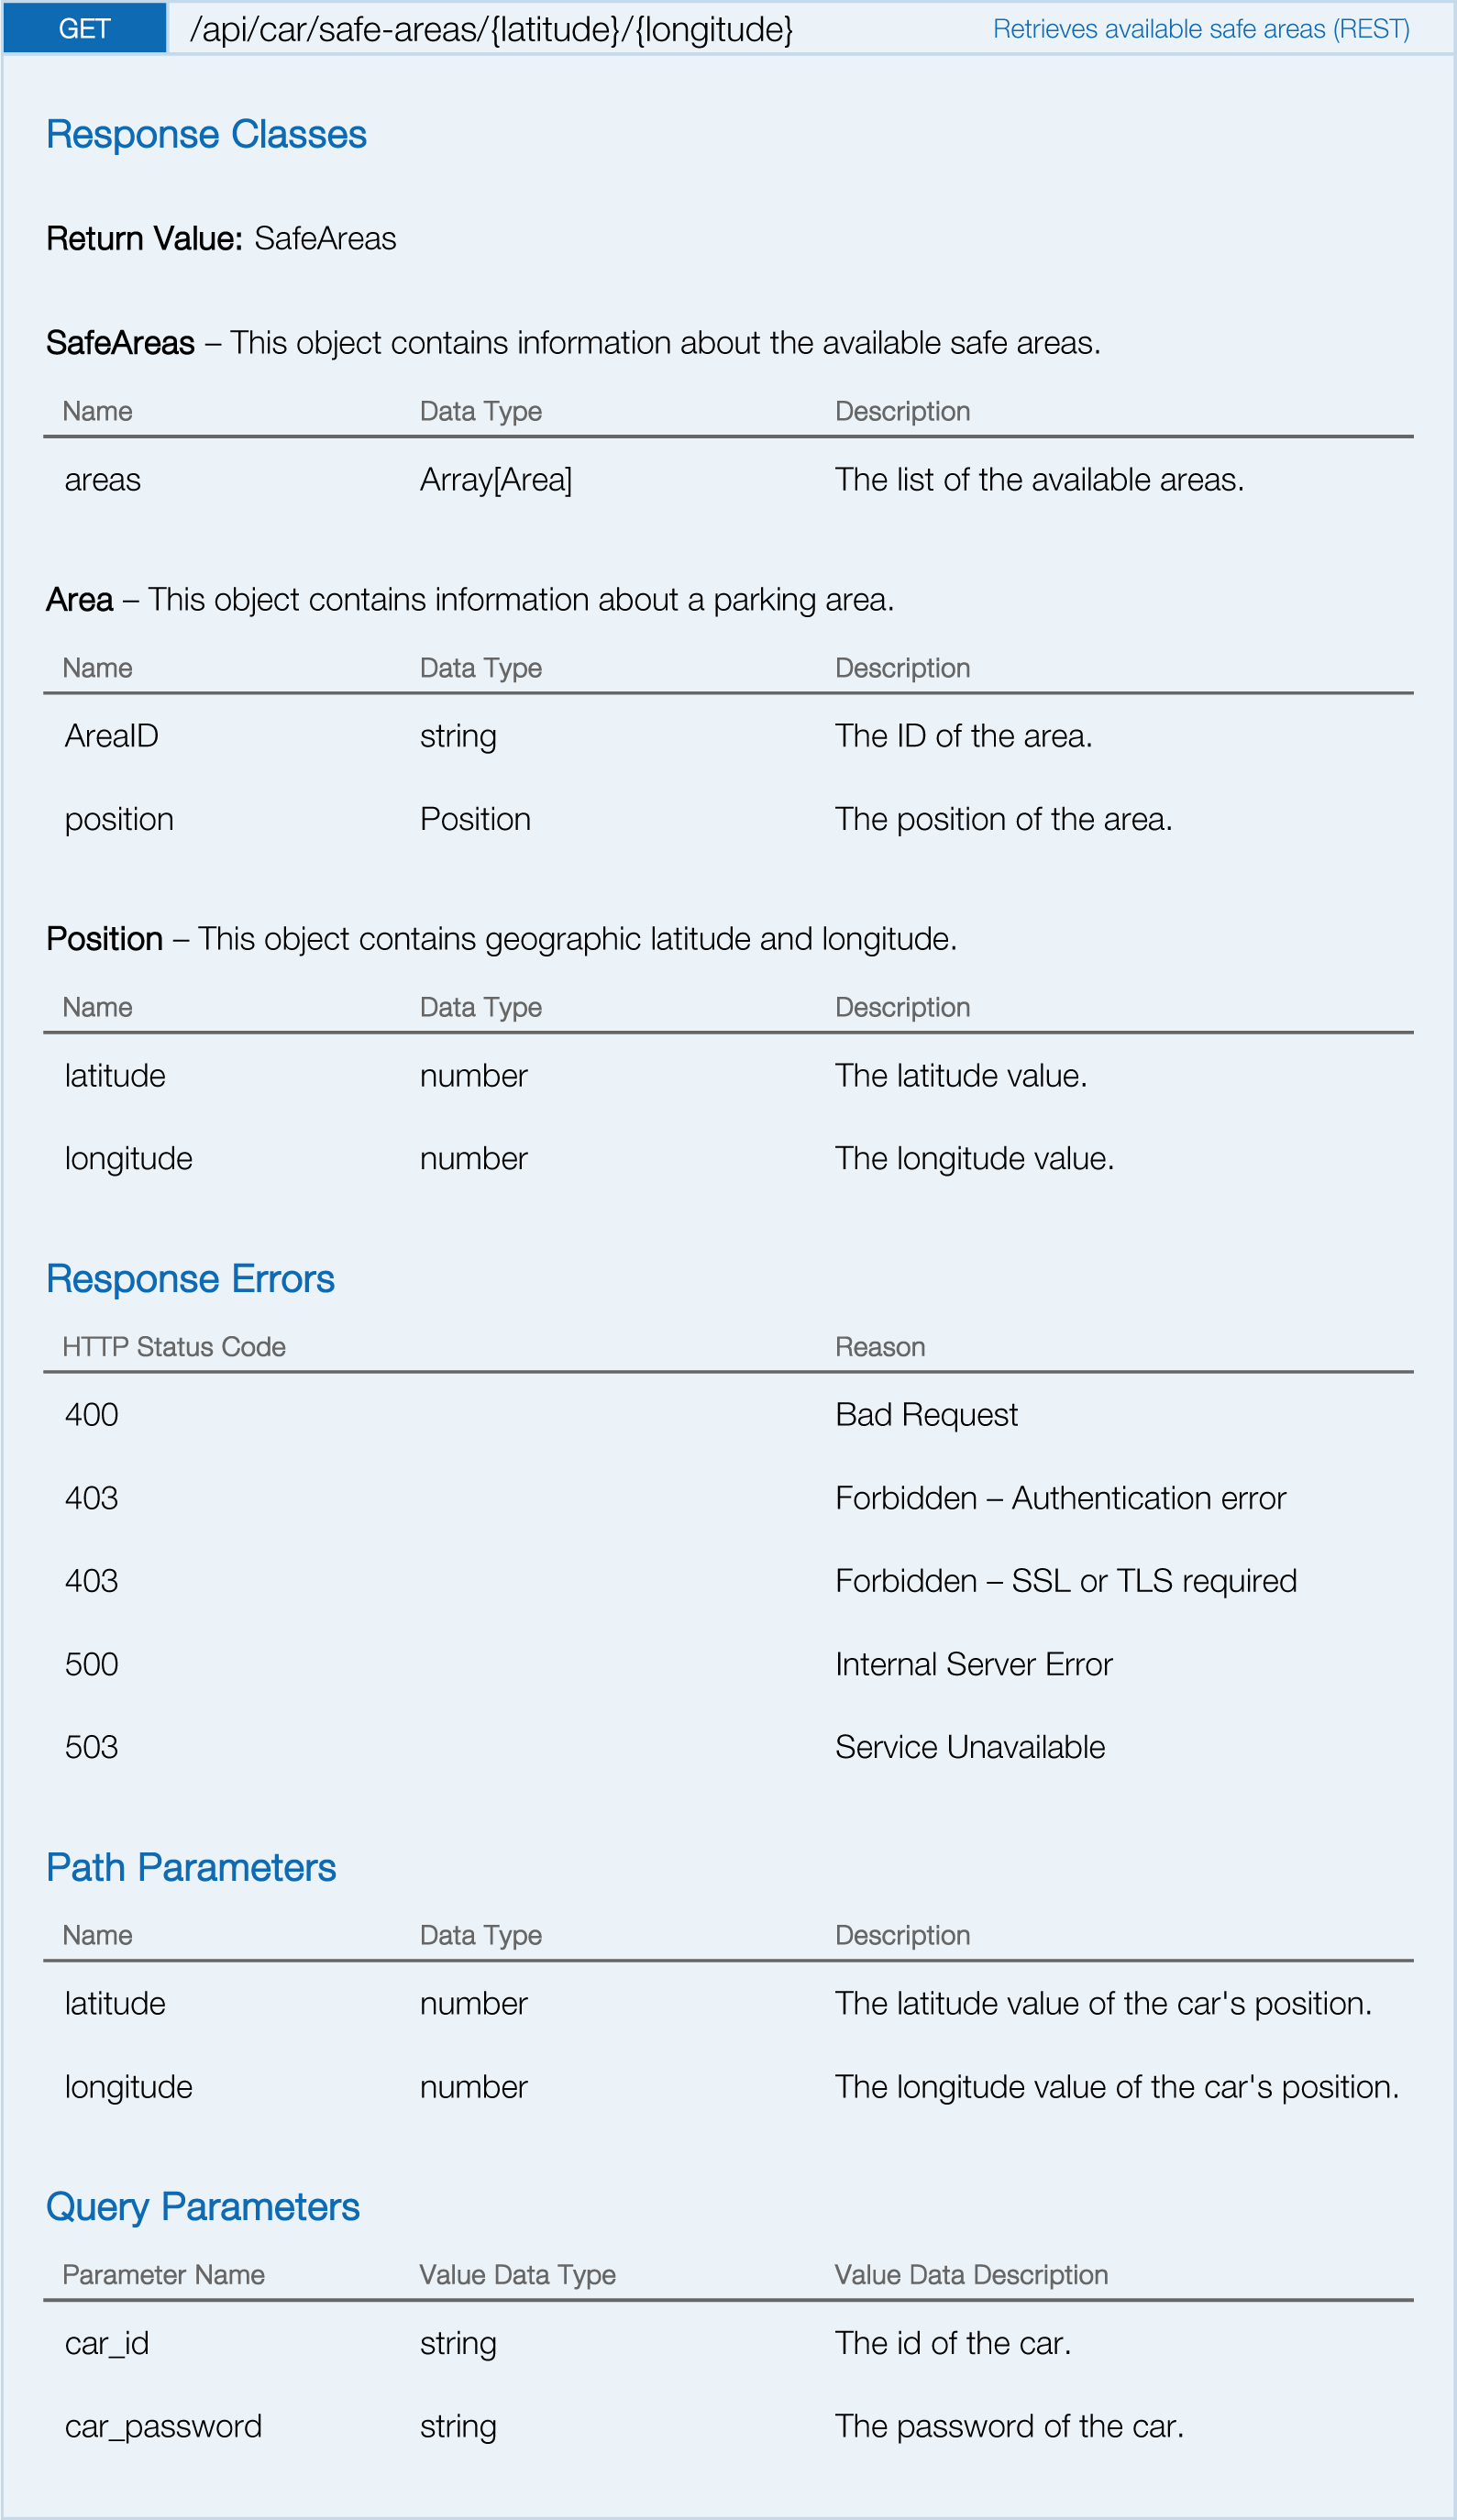
\includegraphics[height=550px, keepaspectratio]{apitables/APISafeAreas.png}
    	\label{fig:api-safe-areas}
\end{figure}

\subsubsubsection{Other requests}

There are other requests, but they are not relevant as the previous requests. For instance:

\begin{itemize}
	\item user's information updating.
	\item payment execution.
	\item current charging information retrieval.
	\item car information retrieval.
\end{itemize}

\subsubsection{Web server to browser}

The users' browsers communicate with the web server via HTTPS requests. Any unencrypted request will be denied.

\subsubsection{External interfaces}

The application server has two external interfaces:
\begin{description}
	\item[SMSGateway:] to send SMS to users.
	\item[PaymentGateway:] to execute credit card payments of users.
\end{description}

\subsection{Runtime view}

The dynamic behaviour of the system is described through sequence diagrams. The following diagrams highlight the most interesting functionalities of the system.

\begin{figure}[H]
	\noindent
    	\centering
    	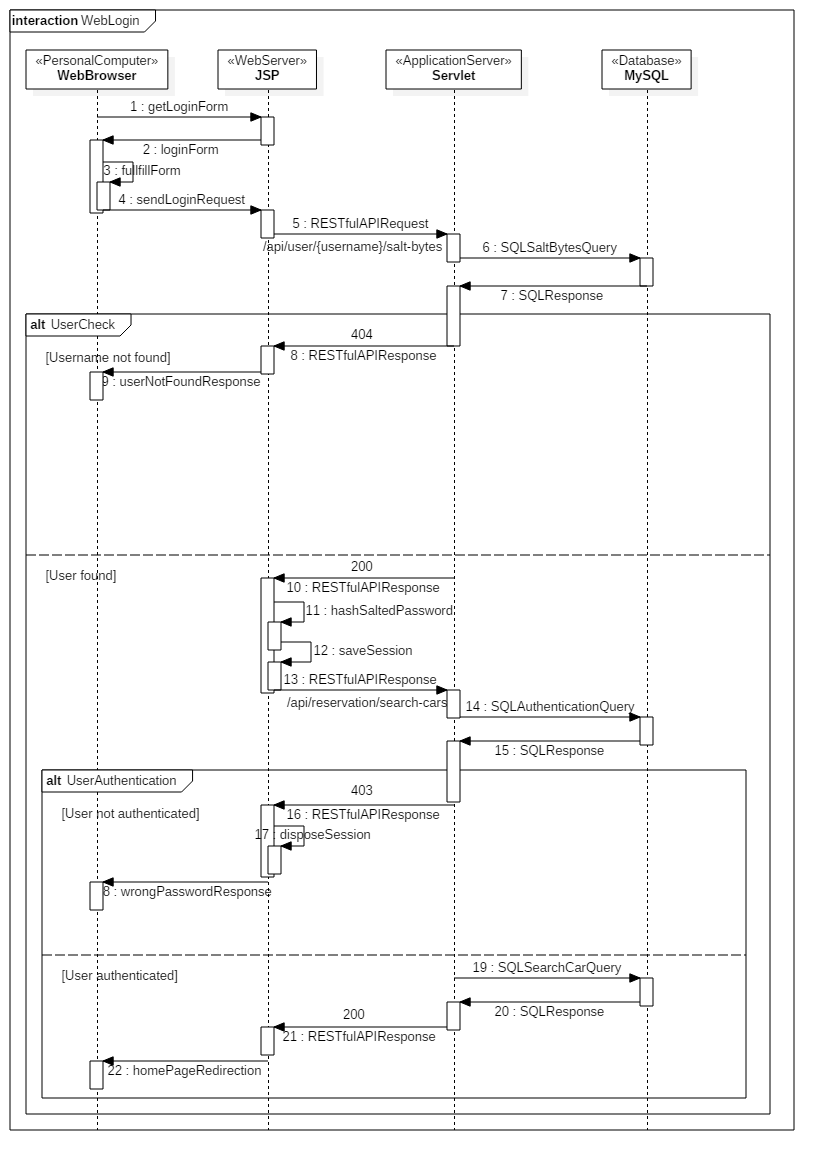
\includegraphics[height=550px, keepaspectratio]{diagrams/SequenceLogin.png}
	\caption{Sequence diagram of the login through the web interface.}
    	\label{fig:sequence-login}
\end{figure}


\begin{figure}[H]
	\noindent
    	\centering
    	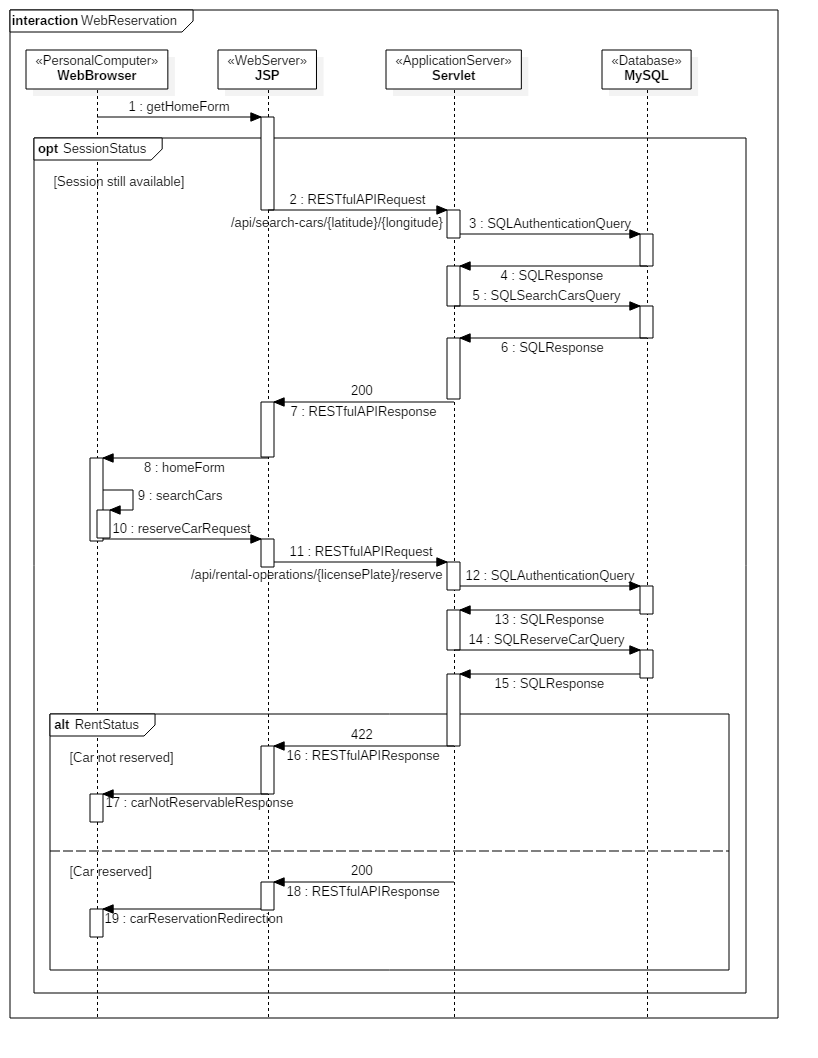
\includegraphics[height=550px, keepaspectratio]{diagrams/SequenceReservation.png}
	\caption{Sequence diagram of the reservation through the web interface.}
    	\label{fig:sequence-reservation}
\end{figure}

\begin{figure}[H]
	\noindent
    	\centering
    	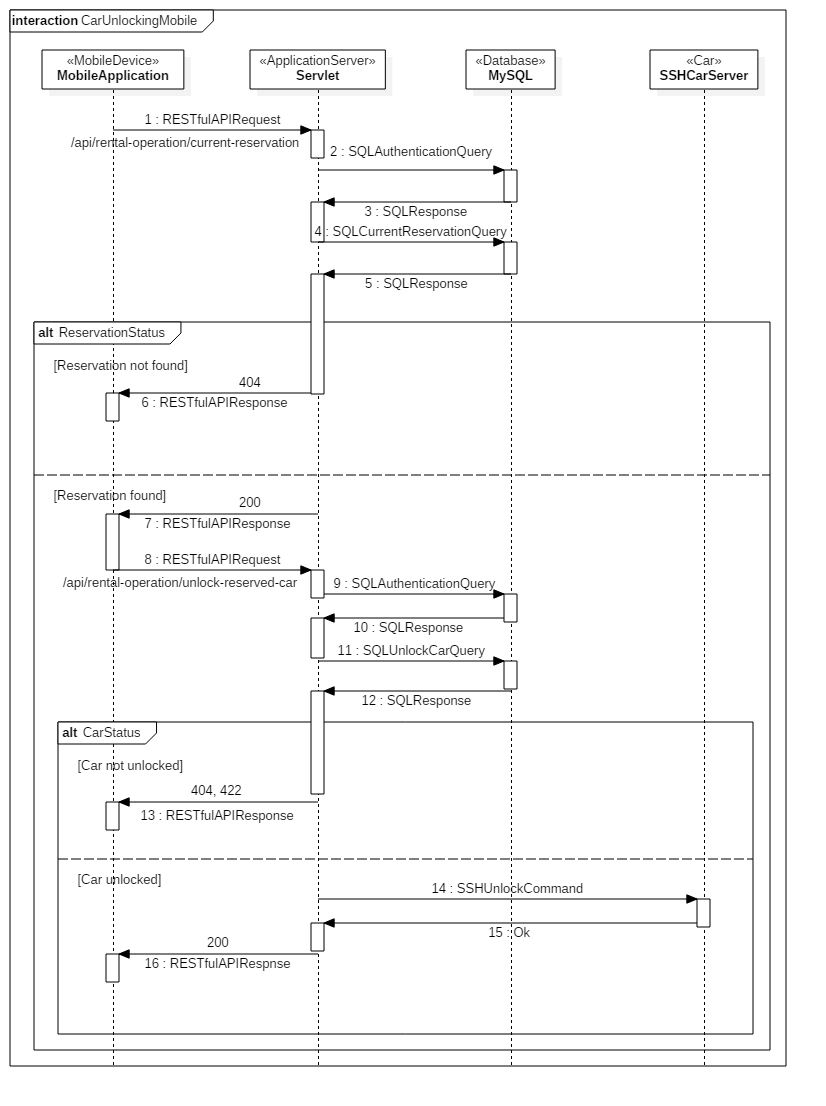
\includegraphics[height=550px, keepaspectratio]{diagrams/SequenceCarUnlocking.png}
	\caption{Sequence diagram for car unlocking through the mobile application.}
    	\label{fig:sequence-unlocking}
\end{figure}

\begin{figure}[H]
	\noindent
    	\centering
    	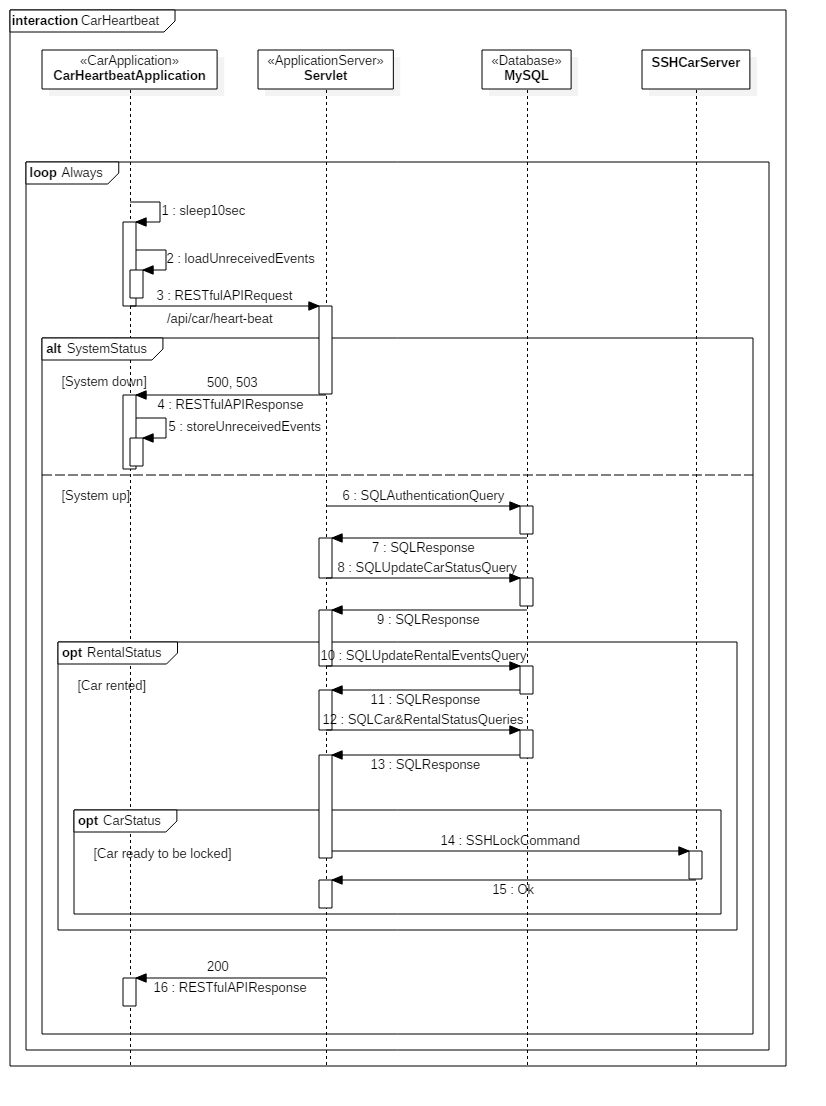
\includegraphics[height=550px, keepaspectratio]{diagrams/SequenceCarHeartbeat.png}
	\caption{Sequence diagram of the car heartbeat process and car locking.}
    	\label{fig:sequence-heartbeat}
\end{figure}

\subsection{Why this architecture}

A good starting point, as an inexperienced software designer, was to keep the level of abstraction of my software as high as possible. That's why, once defined the different logical layers, I chose a multitier architecture with a logical layer per physical tier.

The choice of the REST architectural style increased the level of abstraction of the entire software architecture and brought properties like:

\begin{description}
	\item[Performance:] application server doesn't save any session, so, after replied to a request, is ready to reply to a new request from a different user. The number of active threads is equal to the number of requests that the application server is processing.
	\item[Scalability:] it's possible to add new components without modifying those that already exist.
	\item[Simplicity:] the RESTful API is an uniform interface.
	\item[Modifiability:] it's simple to modify the components. 
	\item[Portability:] components are duplicated easily.
	\item[Reliability:] if there are more web servers, application servers and databases, the system will be able to provide the service even if a component fails.
\end{description}

Last but not least, Java EE offers a set of components that hugely increased the level of abstraction.